  \documentclass[12pt]{article}

\usepackage{amsmath}
%\usepackage{amssymb}
\usepackage{array}
\usepackage{bbm}
\usepackage{booktabs}

%\usepackage[dvipsnames,svgnames,x11names]{xcolor}
\usepackage[markup=underlined]{changes}
\usepackage{cite}
\usepackage{color}
\usepackage{csquotes}
%put footnotes in the end of the paper
%do not forget to release \theendnotes in the end of the paper
%\usepackage{endnotes}
%\let\footnote=\endnote
\usepackage{epigraph}
\usepackage{hyperref}
\usepackage{footmisc}
\setlength{\footnotesep}{\baselineskip}
\usepackage[margin=1in]{geometry}
\usepackage{graphicx}
\graphicspath{{C:/Users/Danila/Pictures/Thesis/}{figures/}}
\usepackage{tabularx}
\usepackage{tabu}
\usepackage{mathtools}
\usepackage{multirow}
\usepackage[round]{natbib}
\usepackage[section]{placeins}
\usepackage{setspace}
\renewcommand{\footnotelayout}{\protect\doublespacing\normalsize}
\usepackage{soul}
\usepackage{textcomp}
\usepackage{threeparttable}
\usepackage{tikz}
\usepackage{verbatim} 
%\usetikz{decorations.pathreplacing}
\usetikzlibrary{arrows}
\usetikzlibrary{arrows.meta}
\usepackage{pdflscape}


\doublespacing

%https://revenuelaw.state.fl.us/LawLibraryDocuments/2015/04/OTH-119274_History%20of%20Sales%20Tax%20%2004132015.pdf
%http://www.aaec.ttu.edu/ceri/published%20papers/journal%20article/usconsumerpurch05.pdf
%opening




\begin{document}
	
	\title{ \vspace{-2.0cm} The Effect of the Sales Tax on Retail Prices and Employment: Evidence from Exemptions on Clothing}
	\author{Danila Pankov (\href{mailto:dap2rb@virginia.edu}{Email}) \thanks{\protect\doublespacing\normalsize I am grateful to my advisors (Leora Friedberg, William Johnson and John Pepper) for support, advice and suggestions. I thank (i) participants of Bureau of Labor and Statistics and University of Virginia workshops for invaluable feedback, (ii) the Bankard Fund for Political Economy for financial support, (iii) Alberto Gonzales, Steer Foundation and  the Radulovacki Fund for traveling support, and (iv) BLS employees (especially, John Molino) for data assistance. I appreciate outstanding revision work of Niveditha Prabakaran. }} %\medskip\\{\normalsize email: \textit{pankov@virginia.edu}}\medskip\\{\normalsize Department of Economics} \medskip\\{\normalsize University of Virginia}}
	%\medskip\\{\normalsize Department of Economics, University of Xxxxxxxxxx (XXXX)}}	
	
		\maketitle
		%\epigraph{"The last time the [sales] tax went up, in a slightly smaller jump, from 3\% to 5\%, was in 1997. The move tipped a recovering economy back into recession."
			
		%	\emph{The Economist}}
		%quote for Japan recession connected with increase in a sales tax
		%\newpage
		\begin{abstract}
			 \normalsize
			Who benefits from sales tax exemptions on apparel? Using frequent state and local policy revisions of these exemptions and three separate datasets, I identify two entities: consumers and retail employees, the latter group generally ignored in the previous research. Addressing endogeneity of the tax policy with respect to business cycles in a difference-in-differences empirical framework, I precisely estimate that a 5 p.p. sales tax exemption fully passes onto consumers and increases employment in the retail apparel sector by 2\%. Consistent with both results simultaneously, I find that apparel demand is quite elastic, supply – super elastic and  average deadweight loss \textemdash 17\textcentoldstyle{}. 
		\end{abstract}
		
	\strut

	\textbf{Keywords:} Sales Tax, Tax Incidence, Labor Expenditures.


	\textbf{JEL Classification Numbers:} H22, H25, H26, J30.
		
		\newpage
		\section{Introduction}
		
		%States and localities broadly use exemptions and exclusions in sales tax to boost economic activity in certain industries or, even, areas. The legislators generally argue that lower tax rate decreases prices faced by consumers and create new jobs. To a certain degree these two goals are countervailing. If consumers are the actual payers of the sales tax, their demand should be relatively inelastic. Thus, exempting the good is unlikely to boost output and, hence, employment. 
		
		Good-specific exemptions are a common part of sales tax policy. 
		When discussing an exemption on a certain good, policymakers generally agree that higher tax rates increase consumer prices and decrease local retail employment but debate the magnitudes of these effects. Economics literature lacks estimates of the effects for commonly exempted goods (groceries, clothing, medical drugs, etc). This paper fills in this gap for apparel, a good on which households spend around 3\% of their incomes and for which the demand is quite elastic \citet{hu, agarwals,einav}.\footnote{\citep{aguiar} shows that apparel is complementary-to-work good, which makes this paper interesting from the optimal tax theory perspective too} Consistent with theory, I find that the tax on apparel generates substantial dead-weight loss: it fully propagates to consumer prices and simultaneously generates large drops in employment. 
		
		%A number of goods is partially or fully exempt from a sales tax. OTT suggests that the higher the tax-induced distortions are in the market, the lower should be the tax rate. Public policy discussion usually emphasizes two main distortions: increase in sales tax results in lower employment and higher prices for consumers. I consider the exemptions on apparel, a policy subject to a constant revision in a number of states. I
		 
		%Setting good-specific sales tax rates through exemptions and other instruments is a substantial part of the sales tax policy in the US. Economic theory suggests that the tax rate on a good should  decrease in the level of tax-induced distortions. When arguing for a lower than general tax rate for apparel, state and locality legislators pay particular attention to two distortions: prices for consumers and number of jobs. Yet  there is lack of empirical literature quantifying these distortions for a number of goods. I fill in this gap for the apparel, expenditures on which comprise 3\% of household incomes, by answering two questions. How large is the pass-through rate of a sales tax on retail prices? How do retailers adjust their inputs, particularly labor, in response to a tax-induced drop in output? 
		
		For my estimation, I employ differences-in-differences empirical strategy. I base it on frequent and sizable apparel-specific tax rate changes induced by  exemptions revisions which state and local governments of Connecticut, New York and Vermont implemented from 2000 to 2012. In my sample, the three states altered their exemptions 10 times, changing the sales tax rate on apparel by 4 to 7 percentage points. Employing these changes for identification have several advantages over variation in the general sales tax rate. First, the changes are large enough for the market participants to recognize them. Second, they affect only the apparel market, rendering general equilibrium effects negligible and having no impact on the precises of the other goods.
		
		%This paper contributes to economic literature by precisely estimating the effects of apparel-specific sales tax on retail prices and employment. First, I use very detailed, item-level, confidential Consumer Price Index micro data to find that the pass-through rate of a sales tax on retail prices is zero. This result is common for the markets of many other goods, but surprising for apparel with its well-documented high elasticity of demand (high responsiveness of consumer expenditures to price changes). A retailers' no-response in price dimension indicates an even more elastic supply. This makes it more interesting to explore how sales tax rate affect the equilibrium usage of inputs, particular employment. Indeed, my estimation shows that a one percentage point decrease in a cumulative state and local sales tax rate implies an 0.33\% increase in employment.
		
		
		On the other hand, employing the exemption alterations exacerbates the traditional identification problem with estimating the effect of sales tax on prices or employment which is spurious correlation between a state's economic conditions and its tax policy changes. Negative shocks to a state economy may simultaneously lower the outcome variable and increase the budget deficit which, in turn, forces legislators to impose higher tax rates. I solve this problem differently for prices and employment. 
		
		In the price case, I take advantage of a typical for exemptions rule which applies zero tax rate for items priced below a certain threshold and full tax rate for the those priced above. A threshold usually equals \$110 but can be as low as \$50. The rule allows me to introduce a third difference in my empirical strategy, with the items priced above the threshold serving as a control group for price trends in the state. To address the endogenous by nature selection of items into the control and treatment groups, I construct an instrument for the tax rate. In the control states, the instrument equals the tax rate itself. In the treatment ones, it is a would-be tax rate based on a price predicted from the prices of the similar clothing items in the control states. 
		
		% My results are robust to different threshold levels that are instituted in different states, and I argue later on that the non-exempt items offer a useful control group.  I also show that pricing around the threshold is not responsive to changes in the threshold value, and I use an IV strategy to deal with the spurious correlation between prices and tax rates. 				
		
		
		
		To this solid foundation for identification, I add detailed, item-level, confidential data from the Consumer Price Index on apparel prices. The data is a panel and has information on certain item characteristics which allows me to identify similarities between items in the control and treatment states and, thus, to implement the triple difference IV empirical strategy for estimating the apparel-specific sales tax effect on pre-tax prices, i.e. the \emph{pass-through rate}.\footnote{Under the assumption of perfect competition, this pass-through rate coincides with tax incidence on producers} I find that the pass-through rate is tightly estimated to be close to zero for most types of apparel, implying that consumers fully bear the burden of the tax. For the apparel market, my result differs from \citet{besley}, who finds overshifting of the sales tax on certain types of apparel, and coincides with the earlier estimate of \citet{poterba}. Both papers use city-level price data and general sales tax rate as a source of variation. 
		
		
		
		
		%The zero pass-through rate is surprising for the apparel industry because it implies that the supply is substantially more elastic than demand, at least, under the assumption of perfect competition.\footnote{} However, previous research \citep{einav,hu}, shows that consumers are quite responsive to the sales tax. ToIn the absence of good data on overall retail sales, I use two implicit ways of checking whether the theoretical prediction holds. First, I check if sales tax increase leads to a lower probability of encountering shortages (temporarily absent items from the shelves) or smaller variety (permanently absent items from the shelves). Luckily, CPI data set thoroughly documents why a certain item is missing from the shelves. Using this information, I find that sales tax does not affect the frequency of encountering any type of missing observations. 
		
		The zero pass-through rate is common for a few other goods (cigarettes \citep{decicca, harding}, alcohol \citep{kenkel}, gas \citep{doyle}, hybrid cars \citet{sallee}, etc.) but surprising for apparel, with its well-documented high elasticity of demand \citep{einav,hu}.\footnote{In the goods market, there are some goods with a positive pass-through rate: diesel fuel \citep{marion, kopczuk} and cars \citep{carbonnier}. For services, the positive pass-through rate is pretty common: haircuts \citet{koponen} and repair services \citep{carbonnier}}. It suggests an even more elastic supply and, hence, a substantial decrease in quantity produced.\footnote{Throughout my paper, I assume perfect competition because none of my results contradicts it. \citep{csen} shows evidence that apparel industry indeed is pretty competitive} This makes it interesting to explore how the sales tax rate affects the equilibrium usage of inputs. 
		
		After merging the sales tax exemptions with data from the Quarterly Census of Employment and Wages, I find that local apparel retailers decrease the number of employees by 0.4\% and the overall expenditures on them by 0.6\%, following a one percentage point increase in the good-specific sales tax rate. 
		This result is quite large: it implies that a New York state 4\% sales tax exemption on clothing results in more than 2,150 new jobs, which is close to the average county employment in the apparel retail sector. Given that the average unemployment duration is 27 months in the sales industry according to the Census, the NY state history of permanent exemption alterations may have resulted in substantial costs. 
		
		When estimating the effect of the sales tax on employment, I do not have an in-state control group as I do in the case of pass-through estimation. To argue that spurious correlation between the sales tax and employment does not drive my results, I perform a robustness check where I use employment in retail stores selling goods for entertainment  instead of clothing and do not find a negative effect of the sales tax changes.  
		
		%DWL
		
		The large effect of sales tax on the apparel retail employment implies that a sales tax substantially reduces the equilibrium quantity of sales in the market and, hence, social welfare. I use the Consumer Expenditure Survey to arrive at my third key result, about deadweight loss. Data on apparel purchases has two limitations: it does not provide detailed geographical information about the consumer or information on whether a certain transaction occurs online or offline. I employ the estimates from \citet{einav} as a proxy for changes in the Internet purchases. Using \citet{goulder}, I find that a 5\% sales tax rate generates a 17\textcentoldstyle{} loss for every tax dollar collected.
		
		There are two major contributions of my paper to economic literature. First, I estimate the pass-through rate of an apparel-specific sales tax on prices using item-level data and variation in the sales tax rate induced by alterations in exemptions. This extends the previous analysis of the influence of the sales tax on the apparel market \citep{besley, poterba}. Second, I am the first to establish the link between the good-specific sales tax and retail employment.  This result adds to a thin literature that explores the effect of the general sales tax rate on employment. While \citet{fox} and \citet{harden} find no effect, \citet{thompson} and \citet{rohlin} show that the effect is present for teh border counties under certain conditions.  
	
		
		The rest of the paper proceeds as follows. Section \ref{sec:model} gives an overview of tax incidence theory. I also use this section to formulate empirical hypotheses I will later test. In Section \ref{sec:data}, I thoroughly describe the data. Section \ref{sec:empstr} contains the explanation of my empirical strategy. In Section \ref{sec:res}, I present my main results, followed by robustness checks of my pass-through estimation in Section \ref{sec:robche}. In Section \ref{sec:dwl}, I calculate deadweight loss.
		
		
		
		
		
		 
		
		%\section{Evidence on the Effects of Good-Specific Taxation}
		%\label{sec:litrev}
		%This section explains how my paper adds to the empirical literature on the effects of good-specific taxation on prices and employment. I start by describing the literature on the effect of taxes on consumer prices, i.e. tax incidence, which has a one-to-one correspondence with the effect of taxes on retail prices, i.e. the pass-through rate. Throughout my discussion, I stick to the terms pass-through rate on retailers vs. tax incidence on consumers because it (i) clearly denotes whether I refer to consumer or producer prices and (ii) is correct regardless of the assumption about competition. Then, I provide an overview of the few research papers that explore the effect of the sales tax on employment, which I augment with a discussion on the apparel expenditure literature.\footnote{I do not review the papers that study the effect of taxes on sales and purchased quantity of non-apparel markets because this literature is not directly related to my paper. Its recent focus is on tax avoidance issues \citep{merri, beatty}}
		
		
		%Start with describing literature on tax incidence: measure the parameter itself + getting more intuition through explaining demand/supply side
		
		%A few empirical papers study tax incidence on prices. I classify them into three categories. The papers from the first category specialize in precisely estimating the tax incidence parameter for a given market. They usually find that consumers fully pay the tax, which is the case in the gasoline market with a sales tax \citep{doyle}, in the clothing market with a sales tax \citep{poterba}, and the alcohol market with an excise tax \citep{kenkel}. There are two noticeable exceptions to this rule.  First, retailers pay half of the VAT on haircuts in Finland \citep{kosonen}. Second, \citet{besley} shows that the sales tax overshifts on consumers for some grocery items and the type of apparel they consider (underwear). I extend the analysis of \citet{poterba} and \citet{besley} by using more granular data and a cleaner identification strategy. Particularly, I am the first in public economics field to use the CPI confidential micro data.\footnote{The most prominent examples of using this data in other fields are \citet{cortes} and \citet{matsa}}
		
		%My estimates also add to the recently emerging literature which studies the effect of the sales tax on total expenditures \citep{agarwals}, online expenditures \citep{einav} and catalog expenditures \citep{hu} in the apparel market. I consider prices at traditional retailers, so the first paper is the most relevant to my research. The authors find that consumers are very responsive to taxes: a 1\% change in the sales tax rate leads to a 2-6\% drop in total expenditures.\footnote{ The authors use sales tax holidays on apparel as a source of variation in the tax rate. When estimating deadweight loss below, I find my estimate to be similar to the lower bound of their result, which is not surprising given that I employ permanent tax rate changes in my analysis} My finding of zero pass-through on pre-tax prices suggests that one can easily convert their estimates into the demand elasticity. 
		
		%Moreover, their result adds to my argument that a lack of salience is not a concern for my estimation. In their seminal paper, \citet{chetty} provide three criteria
		%for the salience of a tax: (i) high tax rates, (ii) large elasticity of demand and 
		%(iii) high prices for a given item. Indeed, relative to grocery items, apparel purchases 
		%readily meet the last two criteria. For the first criteria, the comparison is also in favor of apparel: though the tax rates are similar in magnitude, the tax rate changes in the apparel industry are large and occur at higher frequency. 
		
		%The papers on tax incidence in the two other categories, which I define respectively as \textit{demand} and \textit{supply} papers, go one step further and explore which characteristics of the two sides of the market affect the tax incidence parameter. The demand papers explore the differences between consumers. \citet{harding} presents evidence that consumer geographical location matters: smokers who live closer to the state border face substantially lower pass-through of an excise tax on cigarettes compared to those in the state interior. In addition,  \citet{decicca} argues that search costs explain the varying  tax incidence across consumers; the authors find that heavier smokers, who have higher benefits from investing time in looking for lower prices, experience lower tax incidence. I contribute to the demand papers literature by estimating sales tax incidence for various apparel groups. First, I find that the sales tax only partially shifts onto consumers who purchase girls clothing and footwear, the demand for which is arguably more elastic. Second, I am the first to consider whether the sales tax pass-through differs across seasonal and non-seasonal goods. Traditional tax incidence literature generally ignores seasonality of goods despite  their surprising price behavior during peak demand \citep{cheva}.
		
		%The supply papers consider how industry characteristics affect tax pass-through rate 
		%through the elasticity of supply. \citet{marion} considers the diesel fuel industry, where the elasticity of supply decreases as the refineries and inventories approach full capacity. They use variation across states in this measure for their research.
		%\citet{carbonnier} compares the elasticity of supply between two industries: cars vs. service. The latter industry is substantially more concentrated
		%and, thus, its supply should be less elastic. Consistent with theory, both papers find 
		%that the more inelastic is supply, the higher is the pass-through rate on producers. My paper is closer to these two supply papers. Theoretically, my pass-through result is only consistent with very elastic supply, which I show indirectly. Both academic papers \citep{csen} and case studies provide evidence that it is indeed the case.\footnote{``The Gap between Company's Domestic and Global Market Positioning'', by Talia Lambar, MBA (April 3,2012)}  Interestingly, despite the inelastic 
		%supply of hybrid vehicles in the US, \citet{sallee} finds full shifting of the tax on consumers.\footnote{In this case, a tax credit is a subsidy. The discrepancy of 
		%	\citet{marion} and \citet{sallee} together with recent evidence of consumer's 
		%	differential response to small tax and subsidy \citep{homonoff} suggests that 
		%	one should be cautious of using them interchangeably. This is the main reason I
		%	do not describe economic literature on subsidy incidence in this review} 
		%The other empirical finding in the supply literature is that the pass-through rate
		%depends on the stage where the state collects tax \citep{kopczuk}.
		%https://bizebeebuzz.wordpress.com/tag/herfindahl-index/ - link for public evidence
		
		
		%Elastic supply implies that firms easily adjust their output and, hence, inputs. Confirming this mechanism, I find that apparel sales taxes decrease employment in the retail industry. To the best of my knowledge, this is the first paper that establishes a link between labor employed to produce a good and a tax rate on the good. It adds to a thin literature that explores the effect of the general sales tax rate on employment. While \citet{fox} and \citet{harden} do not find evidence for it, \citet{thompson} and \citet{rohlin} show that the effect is present for border counties under certain conditions.
	

			\section{Theoretical Background}
			\label{sec:model}
			
			%In this brief section, I show that under perfect competition the zero pass-through rate of the sales tax on retail prices is uninformative about the effects. The intuition is the following. The pass-through rate reflects the ratio of the demand and supply elasticities whereas the dead-weight loss depends on the interaction of the two elasticities. Thus, same pass-through rate may well imply both substantial and negligible effects on social welfare. This argument becomes even more valid under imperfect competition, where the pass-through rate depends on a larger set of parameters as I show in Appendix \ref{sec:ic}. 
			
			%In this brief section, I (a) explain why I follow the assumption of perfect competition throughout this paper and (b) show that, while implying full incidence of the tax on consumers, zero pass-through rate has nothing to say about the tax effect on retail employment.
			
			In this section, I (a) explain how the effects of the sales tax on retail prices and employment depend on demand and supply elasticities under perfect competition and (b) show that only elastic demand and super elastic supply can justify my empirical results. In the end, I explain my choice of the perfect as opposed to imperfect competition framework.
			
			In the first column of Table \ref{tab:compstat}, I show how the pass-through rate depends on the ratio of the supply and demand elasticities. Zero or close to zero pass-through rate is plausible when the supply elasticity is substantially larger in magnitude than the demand one: $\epsilon_S>>\epsilon_D$. In Figure \ref{fig:pq}, where I illustrate a zero pass-through rate, I draw an absolutely elastic supply curve (red line). 
			
			Under the assumption of a strictly increasing in labor production function, the employment effect is an increasing function of the quantity effect, $g(.)$. If $\epsilon_S>>\epsilon_D$, the employment effect is proportional go $g(\epsilon_D)$. Thus, a large employment effect implies elastic demand. In Figure \ref{fig:pq}, I show that elastic demand (blue line) leads to a substantially larger quantity effect, and, therefore, employment effect, compared to inelastic demand (green line): $Q_\tau-Q_e$ >> $Q_\tau-Q_i$.
			
			Acknowledging the fact that apparel market may be imperfectly competitive, I stick to the assumption of perfect competition due to two reasons. First, throughout my estimation, I can not reject the hypothesis that the pass-through rate is out of the interval consistent with perfect competition. Note that according to the formula in Table \ref{tab:thr} the interval is $[-1,0]$, whereas under imperfect competition the pass-through rate can also be positive. Second, should the competition be imperfect, the computed in this paper dead-weight loss would be a lower bound of the actual one, making the argument of costly apparel taxation stronger.
			
			%To illustrate the latter statement, I use Figure \ref{fig:wl}. 
			
			
			%Under the assumption of perfect competition, I explain how the effects of the sales tax on prices and quantity, and, therefore, employment, depend on demand and supply elasticities. I show that, while implying full incidence on consumers, zero pass-through lacks information on the magnitude of the tax impact on output, employment or social welfare. %The intuition is the following. The pass-through rate reflects the ratio of the demand and supply elasticities whereas the dead-weight loss depends on the interaction of the two elasticities. Thus, same pass-through rate may well imply both substantial and negligible effects on social welfare. This argument becomes even more valid under imperfect competition, where the pass-through rate depends on a larger set of parameters as I show in Appendix \ref{sec:ic}. 
			
			%Mathematically, the pass-through rate depends on demand and supply elasticities according to the formula in the first column of Table \label{tab:compstat}. Assuming positive supply elasticity and negative demand one, the pass-through belongs to $[-1,0]$ interval. The employment effect is a increasing function of the multiplication between supply elasticity and the pass-through rate. Thus, it is negative but can be of any magnitude.
			
			%Comparative statics generalizes this result. One can always increase the magnitudes of the elasticities so that the pass-through stays constant while the employment effect increases freely. Consider the case when the pass-through rate is close to zero. I can reach any value of the employment effect by proportionally increasing the magnitudes of two elasticities.
			
			
		\begin{table}
			\caption{Comparative Statics of the Sales Tax Effects on Prices and Employment}
			\label{tab:thr}%
			\centering
			\begin{tabular}{cccccc}
				\hline 
				& (1) & (2) & (3) & (4) &  (5) \\
				Effects on & Formula & \multicolumn{2}{c}{Comp. Statics} & \multicolumn{2}{c}{Special Cases}  \\ 
								\hline 
				 & & $|\epsilon_D| \uparrow$ & $\epsilon_S \uparrow$ & $\epsilon_S >> \epsilon_D$ & $\epsilon_D >> \epsilon_S$   \\ 
				%\hline 
				Producer Prices & $=1/(\epsilon_S/\epsilon_D-1) \in [-1,0]$ & $\downarrow$  & $\uparrow$ & $\rightarrow 0$  & $\rightarrow 1$     \\ 
				%\hline 
				Employment & $\sim g(\epsilon_D\epsilon_S/(\epsilon_S-\epsilon_D)) \le 0 $ & $\downarrow$  & $\downarrow$ & $ \sim g(\epsilon_D)$ & $ \sim g(\epsilon_S)$ \\ 
				\hline 				\end{tabular} 
		\end{table}	
			
			
			
			%Figure \ref{fig:pq} illustrates this idea in the output market. When the supply is absolutely elastic, the pass-through rate is zero as long as the demand elasticity is finite. However, the demand elasticity determines output and employment effects. Elastic demand (blue line) leads to substantially larger effect compared to elastic demand (green line): $Q_\tau-Q_e$ >> $Q_\tau-Q_i$.
			
			
			
			%Figure \ref{fig:wl} illustrates this idea in the labor market. When the sales tax is in place, the intersection of the supply line with the black derived demand line determines the equilibrium number of employees is $L(Q_{\tau})$. Introducing the exemption leads to an increase in the derived demand for labor. Elastic apparel demand leads to higher changes in the derived demand (blue line vs. green) and equilibrium amount of labor employment.
			
			
			
			
			%\begin{equation}
			%\label{eq:salesro2}
			%\rho=-\frac{\epsilon_D}{\epsilon_S+\epsilon_D},
			%\end{equation}
			%where $\epsilon_D \ge 0$ is the absolute value of demand elasticity and  $\epsilon_S \ge 0$ --- supply elasticity. The constraints on the elasticities transmit into the constraints on the pass-through rate itself: $\rho \in [-1,0]$. As I show in Appendix \ref{sec:ic}, under the assumption of imperfect competition, the pass-through rate can take any value. At this moment, I am ready to state that:
			
			%\textbf{Proposition 1.} Producer prices can either increase or decrease in response to a rise in the sales tax. Under the assumption of perfect competition, the pass-through equals the tax incidence and belongs to the interval [-1,0]. 
			
			%In my empirical analysis, the pass-through of a sales tax on producer prices always belongs to the interval [-1,0]. Thus, I stick to the assumption of perfect competition. Under this assumption, the concept of a pass-through rate of sales tax on either consumers or producers is synonymous to the tax incidence. \citet{fabinger} shows that under imperfect competition, they are synonyms only for consumers. For producers, the magnitude of the pass-through rate is a lower bound on the tax incidence magnitude. This is true for dead-weight loss as well. Thus, I consider my estimates of the pass-through rate and deadweight loss as conservative.
			
			
			%Deadweight loss depends on the equilibrium quantity response of a sales tax. 
			%\label{eq:salesro}
			%In my empirical analysis, I estimate tax incidence for different groups of apparel separately because the elasticities of demand and supply are likely to vary across these groups. So, I establish the comparative statics of the pass-through rate on producer prices with respect to the demand and supply elasticities. Formula (\ref{eq:salesro2}) suggests that:
			
			%\textbf{Proposition 2.} The pass-through of sales tax on producer prices increases in the elasticity of demand and decreases in the elasticity of supply.
			
			
			\begin{figure}
				\centering
				
				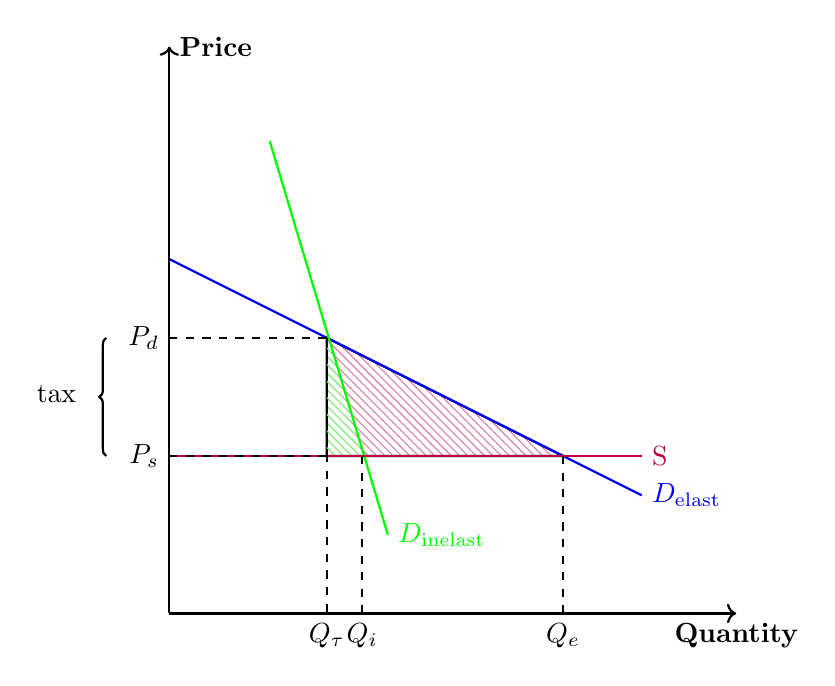
\begin{tikzpicture}[domain=0:6,scale=1,thick]
				\usetikzlibrary{calc}                                %allows coordinate calculations.
				\usetikzlibrary{decorations.pathreplacing}           %allows drawing curly braces.
				\usetikzlibrary{patterns} 
				% Define linear parameters for supply and demand
				\def\dint{4.5}      %Y-intercept for DEMAND.
				\def\dslp{-0.5}     %Slope for DEMAND.
				\def\ditwo{10}
				\def\dstwo{-10}
				\def\sint{2}      %Y-intercept for SUPPLY.
				\def\sslp{0}      %Slope for SUPPLY.
				
		
				\def\tax{1.5}       %Excise (per-unit) tax
				
				% Define Supply and Demand Lines as equations of parameters defined above.
				\def\demand{\x,{\dslp*\x+\dint}}
				\def\supply{\x,{\sslp*\x+\sint}}
				\def\demandtwo{\x,{\dstwo*\x+\ditwo}}
				%\def\supplytwo{\x,{\sslp*\x+\sint+\ssh}}
				
				
				% Define coordinates.
				\coordinate (ints) at ({(\sint-\dint)/(\dslp-\sslp)},{(\sint-\dint)/(\dslp-\sslp)*\sslp+\sint});
				\coordinate (ep) at  (0,{(\sint-\dint)/(\dslp-\sslp)*\sslp+\sint});
				\coordinate (eq) at  ({(\sint-\dint)/(\dslp-\sslp)},0);
				\coordinate (dint) at (0,{\dint});
				\coordinate (sint) at (0,{\sint});
				
				\coordinate (teq) at  ({(\sint+\tax-\dint)/(\dslp-\sslp)},0); %quantity
				\coordinate (tep) at  (0,{(\sint+\tax-\dint)/(\dslp-\sslp)*\sslp+\sint+\tax}); %price
				\coordinate (tint) at  ({(\sint+\tax-\dint)/(\dslp-\sslp)},{(\sint+\tax-\dint)/(\dslp-\sslp)*\sslp+\sint+\tax}); %tax equilibrium
				
				\coordinate (sep) at (0,{\sslp*(\sint+\tax-\dint)/(\dslp-\sslp)+\sint});
				\coordinate (sen) at ({(\sint+\tax-\dint)/(\dslp-\sslp)},{\sslp*(\sint+\tax-\dint)/(\dslp-\sslp)+\sint});   
				
				
				
				% Shade orange area underneath curve.
				\draw[pattern=north west lines, pattern color=purple!50] (2,3.5) -- (2,2) -- (5,2) -- cycle;
				\fill [pattern=north west lines, pattern color=green!50] (2,3.5) -- (2,2) -- (2.45,2) -- cycle;
				
				
				% DEMAND
				\draw[thick,color=blue] plot (\demand) node[right] {$D_{\text{elast}}$};
				
				% DEMAND2
				\draw[thick,color=green] (1.275,6) coordinate (a_1) -- (2.775,1) coordinate (a_2) node[right] {$D_{\text{inelast}}$};
				
				% SUPPLY
				\draw[thick,color=purple] plot (\supply) node[right] {S};
				
				% Draw axes, and dotted equilibrium lines.
				\draw[->] (0,0) -- (7.2,0) node[below] {$\textbf{Quantity}$};
				\draw[->] (0,0) -- (0,7.2) node[right] {$\textbf{Price}$};
				\draw[decorate,decoration={brace},thick]  ($(sep)+(-0.8,0)$) -- ($(tep)+(-0.8,0)$) node[midway,below=-8pt,xshift=-18pt] {tax};
				
				\draw[dashed] (tint) -- (teq) node[below] {$Q_\tau$};
				\draw[dashed] (2.45,2) -- (2.45,0) node[below] {$Q_i$};
				\draw[dashed] (5,2) -- (5,0) node[below] {$Q_e$};                  
				\draw[dashed] (tint) -- (tep) node[left] {$P_d$};                       
				\draw[dashed] (sen) -- (sep) node[left] {$P_s$};                        
				
				
				\end{tikzpicture}
				\caption{Comparison of deadweight losses when pass-through rate is zero}
				\medskip
				\begin{minipage}{1\textwidth}
					{ \small \emph{Notes:} Deadweight loss generated by a sales tax is substantially larger when demand is elastic (blue line) rather than inelastic (green line). In the former case, the deadweight loss is all the shaded area, whereas in the latter --- the green shaded area}
				\end{minipage}
				\label{fig:pq}
			\end{figure}
			
			\begin{comment}
			In addition to changing the prices, the sales tax may also decrease the equilibrium quantity. This forces firms to employ fewer inputs. The magnitude of this decrease depends on the demand and supply elasticities. In Figure \ref{fig:pq} I show that the output responses increase in the elasticity of demand: $Q_i-Q_\tau<Q_e-Q_\tau$. In Figure \ref{fig:wl}, I depict the corresponding input responses in the elasticity of demand: $L(Q_i)-L(Q_\tau)<L(Q_e)-L(Q_\tau)$. The same result is true for the supply elasticity, which allows me to state: 
			
			\textbf{Proposition 3.} The imposition of a sales tax may lead to a decrease in the equilibrium output, and, hence, inputs employed by suppliers. The higher the elasticities of demand and supply, the larger the decrease.
			
			Note that the deadweight loss of a sales tax also increases with respect to both elasticities. Thus, a large effect on the inputs used by firms signals substantial losses due to the tax.
	
			%Labor market
			\begin{figure}
				\centering
				
				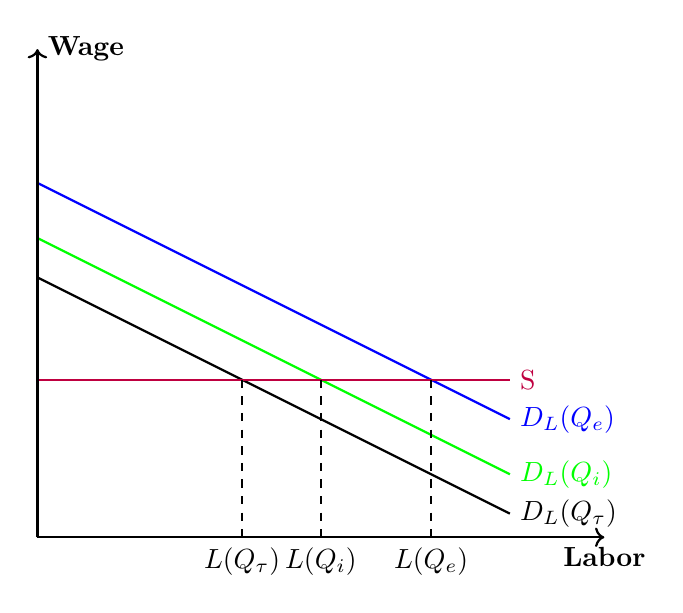
\begin{tikzpicture}[domain=0:6,scale=1,thick]
				\usetikzlibrary{calc}                                %allows coordinate calculations.
				\usetikzlibrary{decorations.pathreplacing}           %allows drawing curly braces.
				\usetikzlibrary{patterns} 
				% Define linear parameters for supply and demand
				\def\dint{4.5}      %Y-intercept for DEMAND.
				\def\dslp{-0.5}     %Slope for DEMAND.
				\def\ditwo{3.8}
				\def\dstwo{-0.5}
				\def\dithree{3.3}
				\def\dsthree{-0.5}
				\def\sint{2}      %Y-intercept for SUPPLY.
				\def\sslp{0}      %Slope for SUPPLY.
				
				
				% Define Supply and Demand Lines as equations of parameters defined above.
				\def\demand{\x,{\dslp*\x+\dint}}
				\def\supply{\x,{\sslp*\x+\sint}}
				\def\demandtwo{\x,{\dstwo*\x+\ditwo}}
				\def\demandthree{\x,{\dsthree*\x+\dithree}}
				
				
				% Define coordinates.
				\coordinate (ints) at ({(\sint-\dint)/(\dslp-\sslp)},{(\sint-\dint)/(\dslp-\sslp)*\sslp+\sint});
				\coordinate (ep) at  (0,{(\sint-\dint)/(\dslp-\sslp)*\sslp+\sint});
				\coordinate (eq) at  ({(\sint-\dint)/(\dslp-\sslp)},0);
				
				
				
				% DEMAND
				\draw[thick,color=blue] plot (\demand) node[right] {$D_L(Q_e)$};
				
				% DEMAND2
				\draw[thick, color=green] plot (\demandtwo) node[right] {$D_L(Q_i)$};
				
				% DEMAND3
				\draw[thick, color=black] plot (\demandthree) node[right] {$D_L(Q_\tau)$};
				
				
				% SUPPLY
				\draw[thick,color=purple] plot (\supply) node[right] {S};
				
				% Draw axes, and dotted equilibrium lines.
				\draw[->] (0,0) -- (7.2,0) node[below] {$\textbf{Labor}$};
				\draw[->] (0,0) -- (0,6.2) node[right] {$\textbf{Wage}$};
				%\draw[decorate,decoration={brace},thick]  ($(sep)+(-0.8,0)$) -- ($(tep)+(-0.8,0)$) node[midway,below=-8pt,xshift=-18pt] {tax};
				
				%\draw[dashed] (tint) -- (teq) node[below] {$Q_T$};
				\draw[dashed] (2.6,2) -- (2.6,0) node[below] {$L(Q_\tau)$};
				\draw[dashed] (3.6,2) -- (3.6,0) node[below] {$L(Q_i)$}; 
				\draw[dashed] (5,2) -- (5,0) node[below] {$L(Q_e)$};        
				
				
				%\draw[dashed] (tint) -- (tep) node[left] {$P_d$};                       
				%\draw[dashed] (sen) -- (sep) node[left] {$P_s$};                        
				
				
				\end{tikzpicture}
				
				\caption{Employment change after tax exemption introduction}
				\medskip
				\begin{minipage}{1\textwidth}
					{ \small \emph{Notes:} Decrease in derived demand for employment generated by a sales tax is substantially larger when demand is elastic (blue line) rather than inelastic (green line). In the former case, the change equals $L(Q_e)-L(Q_\tau)$, whereas in the latter --- $L(Q_i)-L(Q_\tau)$}
				\end{minipage}	
				\label{fig:wl}
			\end{figure}
			
			
			\end{comment}		
			
			
			
			
	\section{Policy Details and Data}
			
	For my empirical analysis, I augment three government-collected data sets with self-collected data on sales tax exemptions and sales tax rates for the Northeast states, resulting into three spanning from January 1997 to December 2012 panels. To estimate the sales tax effect on employment and consumer expenditures, I extract county-level data from the Quarterly Census of Employment and Wages  (QCEW), and household-level data from Consumer Expenditure Survey (CE) respectively. When estimating the pass-through rate, I use item-level Consumer Price Index (CPI) micro data and add the Midwest states to my sample. 
	
	I start this section by showing how alterations in exemptions affect sales tax rates. Then, I describe the data for estimating the price and employment effects, leaving the CE data description for online Appendix \ref{app:ed}. 
	
		 			\begin{table}
		 				\caption{Population Weighted Average Cumulative Sales Tax Rates in Northeast and Midwest States for Apparel by Price Categories}
		 				\label{tab:salestax}
		 				\centering
		 				\begin{threeparttable}	
		 					\begin{tabular}{lccccccccc}
		 						\toprule
		 						& \multicolumn{9}{l}{\textbf{Average Sales Tax Rates in}}  \\
		 						& \multicolumn{7}{c}{Treatment States} & \multicolumn{2}{c}{Control States} \\ 
		 						\cmidrule(r){2-8} \cmidrule(r){9-10}
		 						& \multicolumn{2}{c}{NY} & \multicolumn{3}{c}{CT} & \multicolumn{2}{c}{VT} & IL & Other   \\
		 						\cmidrule(r){2-3} \cmidrule(r){4-6} \cmidrule(r){7-8}
		 						& \multicolumn{7}{c}{for Different Price Categories} & & MW \\
		 						\cmidrule(r){9-9} \cmidrule(r){10-10}
		 						Year & $\le\$110$ & $>\$110$ & $\le\$50$ & $(\$50;\$75]$ & $>\$75$ & $\le\$110$ & $>\$110$ & \multicolumn{2}{c}{for All Prices} \\
		 						\midrule
		 						1997 & 7.91 & 7.91 & 0.00 & 0.00 & 6.00 & 5.00 & 5.00 & 7.48 & 5.32\\
		 						2000 & 1.74 & 7.93 & 0.00 & 0.00 & 6.00 & 0.01 & 5.01 & 7.55 & 5.36\\
		 						2003 & 8.40 & 8.40 & 0.00 & 6.35 & 6.35 & 0.02 & 6.02 & 7.63 & 5.63\\
		 						2006 & 2.34 & 8.27 & 0.00 & 6.35 & 6.35 & 0.02 & 6.09 & 7.68 & 5.67\\
		 						2008 & 2.34 & 8.27 & 0.00 & 6.35 & 6.35 & 0.00 & 0.00 & 7.68 & 5.67\\
		 						2010 & 6.60 & 8.47 & 0.00 & 6.35 & 6.35 & 0.00 & 0.00 & 8.02 & 5.72\\
		 						2012 & 2.44 & 8.47 & 6.50 & 6.50 & 6.50 & 0.00 & 0.00 & 7.60 & 5.77\\
		 						\multicolumn{10}{l}{\textbf{The Northeast control states (MN,MA,NH,NJ,PA,RI) have constant rates}}\\ \noalign{\smallskip}\hline	 
		 					\end{tabular}
		 					\begin{tablenotes}[para,flushleft]
		 						\small \emph{Notes:}  I use December tax rates for each year in the table to compute the average of cumulative tax rates weighted by municipalities population. For the Northeastern states and Illinois, I obtain data on state and local tax rates and exemptions from the state government websites. For the other Midwestern states, I use state and average municipal tax rate weighted by state population from several online sources. ``Other Midwest'' states are Iowa, Indiana, Kansas, Kentucky, Michigan, Minnesota, Missouri, Nebraska, North Dakota, Ohio, South Dakota, Wisconsin. Data on population for states and municipalities are from 2010 Census.
		 					\end{tablenotes}
		 				\end{threeparttable}
		 			\end{table}	
	\subsection{Changes in Sales Tax Rates}
	
	In my sample, alterations to state and local exemptions are the major source of variation in the sales tax rate across time, location and item price. A sales tax exemption on apparel is a policy which makes clothing and/or shoes items priced below a certain threshold tax free. 	
	 In the past two decades, three states have substantially altered their sales tax exemption rules on apparel, defined as clothing plus footwear: Connecticut (twice), New York  (six times) and Vermont (twice).\footnote{Massachusetts and Rhode Island have slightly trimmed their exemption thresholds. See Appendix \ref{app:exm} for the complete list of local and state exemptions alterations.}  As a result, sales tax rates for certain apparel items changed by 4 to 6.5 percentage points. In addition, a few New York localities changed their sales tax rate on apparel from 1.5 to 4.5 p.p. by altering their exemptions.
	
	
	To show how state and local exemptions influence the cumulative tax rate in New York City, I plot the rate on apparel items priced above \$110 and below \$55 in Figure \ref{fig:nyrates}. \footnote{To obtain the rate on middle priced items (\$55-\$110), extend the last spike of the black line till April 2012.} There are three observations from the plot. First, there is at least one exemption every three years. Second, they change the tax rate by at least 4\%. Finally, whereas the first two alterations (2000,2003) coincide in time and in items targeted, the later city exemptions are more generous and last longer.
	
	
	 %Throughout my sample, New York and, until 2007, Vermont, allow its cities and counties to tax or exempt apparel separately. 22 NY counties and 6 NY cities (out of 62 and 61 respectively) have altered these rules at least once, changing the sales tax rate on apparel from 1.5 to 4.5 percentage points. In Vermont, there are 4 such municipalities, which set sales tax of 1 p.p. and comprise less than 10\% of the state population. 
	
	
	
	
	%In this subsection, I describe in detail how the sales tax rate varies for different price 
	%categories in the treatment states and compare it with the variation in the control states. For the Northeast, 
	%I collect the data on state and local sales tax exemptions and the general sales tax 
	%rate from previous and current versions of state government websites. I 
	%find that the only discrepancy between my data and the CPI data occurs due to alternations in the
	%exemptions. Given that there are no apparel-specific exemptions in the Midwest, I use the tax rates from Consumer Price Index micro data for this region.
	
	%A sales tax exemption makes items for a certain price-category tax-free. In the past two decades, four states have changed their sales tax exemption rules on apparel, defined as clothing plus footwear: Connecticut (twice), New York  (six times), Rhode Island (once) and Vermont (twice). I, however, ignore the exemption in Rhode Island because it affects only a small share of apparel items that cost more than \$250.\footnote{Also, the revision in the Rhode Island exemption happens at the very end of my sample: in October of 2012. Such items generally include night dresses, fancy suits, etc.} The other exemptions generate tax rate decreases or increases ranging from 5 to 9 percentage points, and, thus, can substantially influence the behavior of market participants. Note that a given tax exemption affects only a certain, \emph{treated}, group of items in a treatment state, allowing all the other items in the state to serve as a control.

			
	In Table \ref{tab:salestax}, I compare the history of population weighted average cumulative sales tax rates for several price categories in the treatment states (New York, Connecticut and Vermont) and in the control states (the other Northeastern and the Midwestern states). The first two columns of the table show that in New York the items priced below \$110, the most common threshold, face a very volatile tax rate  relative to items priced above, which movement resembles Illinois. 
	
	In Connecticut (Columns (3-5) of Table \ref{tab:salestax}) and Vermont (Columns (6-7)), state legislators have changed the exemption policy twice. Starting from the \$75 threshold in 1997, the Connecticut legislators first decreased the threshold to \$50 in 2003 and then completely repealed the exemption in 2011. On the contrary, Vermont fully taxed apparel at the beginning of my sample. Then, its legislators introduced exemption on clothing with \$110 threshold and extended it to shoes in 2001. In 2007, all apparel became tax free. For some years Vermont cumulative tax rates are not whole numbers because the state allowed four municipalities to impose 1\% local option tax and apply exemptions on clothing to it from 1999 to 2007.  %Connecticut does not allow localities to administer a sales tax --- and in Vermont only four municipalities charge a 1\% additional to state tax before 2007, when the new exemption rules eliminate any tax on clothing.
	%In Vermont, there are 4 such municipalities, which set sales tax of 1 p.p. and comprise less than 10\% of the state population. 
	
	The tax rates in the control states stay almost constant throughout my sample. New Hampshire does not impose any sales tax, whereas Pennsylvania and New Jersey fully exempt clothing from taxation. Maine imposes a constant 5\% cumulative/state tax. In Massachusetts, a 2008 state sales tax increase from 5\% to 6.25\% affects only a small share of items priced above \$175. The same argument applies to Rhode Island's exemption repealed in October 2012 that makes items priced above \$250 taxable. In Illinois (Column 7), there is a tiny increase in the sales tax rate from 7.5\% to 7.6\% in the last two decades, whereas the rest of the Midwest states experience an almost a 9\% increase from 5.32\% to 5.77\%. 
	
	
	
	
	%When New York and, before 2007, Vermont state exemptions are in place, the tax rate is not zero because their localities may opt to continue applying local sales tax rates. In Vermont, the localities have negligibility impact on the cumulative tax rate

		

		\begin{figure}
			\centering
			
			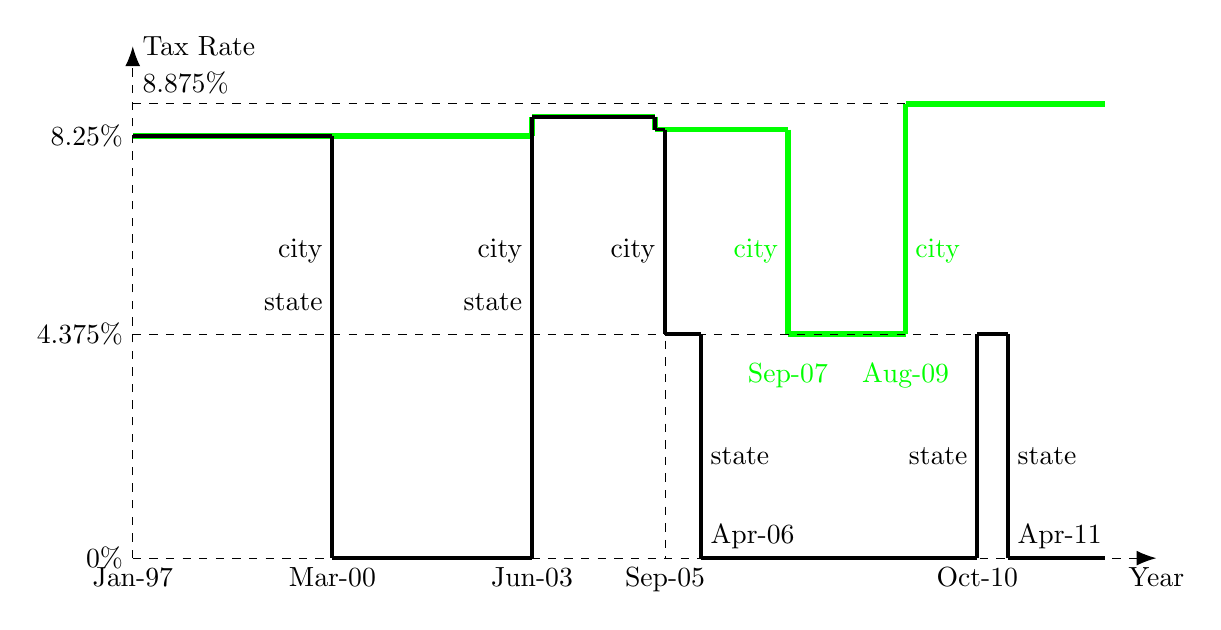
\begin{tikzpicture}[scale=0.65]
			
			% horizontal axis
			
			\draw[dashed,arrows={-Latex[length=2.5mm]}] (0,0) --++ (20,0) node[anchor=north] {Year};
			%labels x axis
			\draw	(0,0) node[anchor=north] {Jan-97};
			\draw	(3.9,0) node[anchor=north] {Mar-00};
			\draw	(7.8,0) node[anchor=north] {Jun-03};
			\draw	(10.4,0) node[anchor=north] {Sep-05};
			\draw	(11.1,0) node[anchor=south west] {Apr-06};
			\draw	(12.8,4) node[anchor=north, green] {Sep-07};
			\draw	(15.1,4) node[anchor=north, green] {Aug-09};
			\draw	(16.5,0) node[anchor=north] {Oct-10};
			\draw	(17.1,0) node[anchor=south west] {Apr-11};
			
			
			% vertical axis
			\draw[dashed,arrows={-Latex[length=2.5mm]}] (0,0) --++ (0,10) node[anchor=west] {Tax Rate};
			%labels y axis
			\draw	(0,0) node[anchor=east] {0\%};
			\draw	(0,4.375) node[anchor=east] {4.375\%};
			\draw	(0,8.25) node[anchor=east] {8.25\%};
			\draw	(0,8.875) node[anchor=south west] {8.875\%};
			
			%labels exemptions
			\draw	(3.9,6) node[anchor=east] {city};
			\draw	(3.9,5) node[anchor=east] {state};
			\draw	(7.8,6) node[anchor=east] {city};
			\draw	(7.8,5) node[anchor=east] {state};
			\draw	(10.4,6) node[anchor=east] {city};
			\draw	(11.1,2) node[anchor=west] {state};
			\draw	(12.8,6) node[anchor=east,green] {city};
			\draw	(15.1,6) node[anchor=west, green] {city};
			
			\draw	(16.5,2) node[anchor=east] {state};
			\draw	(17.1,2) node[anchor=west] {state};
			
			
			
			% >110 TaxRate
			\draw[line width=0.7mm, green] (0,8.25) -- (7.8,8.25);
			\draw[line width=0.7mm, green] (7.8,8.25) -- (7.8,8.625);
			\draw[line width=0.7mm, green] (7.8,8.625) -- (10.2,8.625);
			\draw[line width=0.7mm, green] (10.2,8.625) -- (10.2,8.375);
			\draw[line width=0.7mm, green] (10.2,8.375) -- (12.8,8.375);
			\draw[line width=0.7mm, green] (12.8,8.375) -- (12.8,4.375);
			\draw[line width=0.7mm, green] (12.8,4.375) -- (15.1,4.375);
			\draw[line width=0.7mm, green] (15.1,4.375) -- (15.1,8.875);
			\draw[line width=0.7mm, green] (15.1,8.875) -- (19,8.875);
			% <110 TaxRate
			
			\draw[line width=0.5mm] (0,8.25) -- (3.9,8.25);
			\draw[line width=0.5mm] (3.9,8.25) -- (3.9,0);
			\draw[line width=0.5mm] (3.9,0) -- (7.8,0);
			\draw[line width=0.5mm]  (7.8,0)--(7.8,8.625);
			\draw[line width=0.5mm] (7.8,8.625) -- (10.2,8.625);
			\draw[line width=0.5mm] (10.2,8.625) -- (10.2,8.375);
			\draw[line width=0.5mm] (10.2,8.375) -- (10.4,8.375);
			\draw[line width=0.5mm] (10.4,8.375) -- (10.4,4.375);
			\draw[line width=0.5mm] (10.4,4.375) -- (11.1,4.375);
			\draw[line width=0.5mm] (11.1,4.375)--(11.1,0);
			\draw[line width=0.5mm] (11.1,0) -- (16.5,0);
			\draw[line width=0.5mm] (16.5,0) -- (16.5,4.375);
			\draw[line width=0.5mm] (16.5,4.375) -- (17.1,4.375);
			\draw[line width=0.5mm] (17.1,4.375) -- (17.1,0);
			\draw[line width=0.5mm] (17.1,0) -- (19,0);
			
			%dashed lines
			\draw[dashed] (0,4.375) -- (17.1,4.375);
			\draw[dashed] (0,8.875) -- (15.1,8.875);
			\draw[dashed] (10.4,4.25) -- (10.4,0);
			
			\end{tikzpicture}
			\caption{Cumulative Sales Tax Rate in New York City }
			
			\medskip
			\begin{minipage}{1\textwidth}
				{ \small \emph{Notes:} Green line represents the tax rate for items priced above \$110, whereas black --- below \$55. ``city'' or ``state'' denotes city or state tax exemption change.}
			\end{minipage}	
			\label{fig:nyrates}
		\end{figure}	
		
	
	
	
	

	
	

		
		
		\subsection{CPI Micro Data}
		
		For estimating the pass-through rate, I extract prices and other variables describing apparel items in the Northeast and Midwest Regions from  the confidential Consumer Price Index (CPI) micro data, to which the Bureau of Labor and Statistics has graciously granted me access. 	
		Below, I briefly enumerate the steps to obtain my final data set from the CPI and provide summary statistics for the variables. For the details about CPI data collection and summary statistics on data used in missing observations regressions, I refer the reader to the data Appendices \ref{sec:dcp} and \ref{sec:id} .
		
		CPI is a regionally representative panel where a unit of observation is a quote. The surveyors record prices for every quote monthly or bi-monthly. As Figure \ref{fig:evquote} shows, every quote consists of consequently substituting each other items, or versions. An item is a good sold at a given store. A hypothetic example is a ``Levi's'' gray, 100\% cotton, M-size, men t-shirt displayed at the Gap store with the following address: 543 Madison Avenue, Poughkeepsie, NY.  A surveyor randomly selects an item based on quote type (t-shirts, sweaters), collects detailed information on it, and follows its price. Once the item becomes permanently unavailable, she replaces it with another one.
		

		
				\begin{figure}
					
					
					\centering
					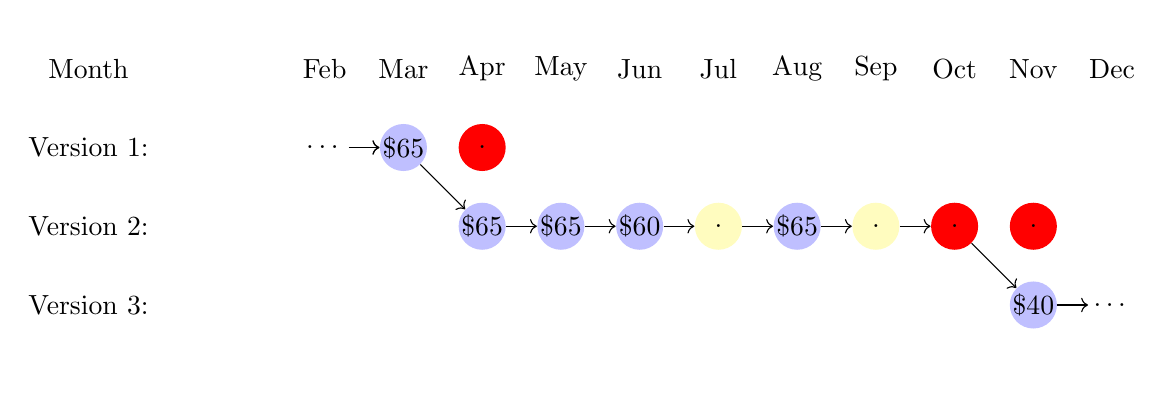
\begin{tikzpicture}%[shorten >=1pt,->]
					
					
					\tikzstyle{names}=[circle,fill=white!25,minimum size=17pt,inner sep=0pt]
					%Months
					\foreach \name/\x in { Month/1, Feb/4, Mar/5, Apr/6, May/7,Jun/8,Jul/9,Aug/10,Sep/11,Oct/12, Nov/13, Dec/14}
					\node[names] (M-\x) at (\x,5) {\name};
					
					%Version1 Row -White Circles
					\foreach \name/\x in { Version 1:/1, \ldots/4}
					\node[names] (V1-\x) at (\x,4) {\name};
					
					%Version1 Row - Blue Circles
					\tikzstyle{vertex}=[circle,fill=blue!25, minimum size=17pt,inner sep=0pt]
					\node[vertex] (V1-5) at (5,4) {$\$65$};
					
					%Version2 Row - First Column
					\node[names] (V2-1) at (1,3) {Version 2:};
					
					%Version2 Row - Blue Circles
					
					\foreach \name/\x in {65/6, 65/7, 60/8, 65/10}
					\node[vertex] (V2-\x) at (\x,3) {$\$\name$};
					
					%Version2 Row - Yellow Circles	
					\tikzstyle{tmisvertex}=[circle,fill=yellow!25,minimum size=17pt,inner sep=0pt]
					\foreach \name/\x in {./9, ./11}
					\node[tmisvertex] (V2-\x) at (\x,3) {$\name$};
					
					%Version2 Row - Red Circles	
					\tikzstyle{tpervertex}=[circle,fill=red!100,minimum size=17pt,inner sep=0pt]
					\foreach \name/\x in { ./12,./13}
					\node[tpervertex] (V2-\x) at (\x,3) {$\name$};
					
					%Version1 Row - Red Circles	
					\node[tpervertex] (V1-6) at (6,4) {$.$};
					
					
					%Version3 Row - White Circles	
					\foreach \name/\x in { Version 3:/1, \ldots/14}
					\node[names] (V3-\x) at (\x,2) {\name};
					
					%Version3 Row - Blue Circles	
					\node[vertex] (V3-13) at (13,2) {$\$40$};
					%Links
					%First row:
					\foreach \from/\to in {4/5,5/6}
					\draw [->] (V1-4) -- (V1-5);
					\draw [->] (V1-5) -- (V2-6);
					\foreach \from/\to in {6/7, 7/8, 8/9, 9/10, 10/11,11/12}
					\draw [->] (V2-\from) -- (V2-\to);
					
					\draw [->] (V2-12) -- (V3-13);
					\draw [->] (V3-13) -- (V3-14);
					%Braces
					%\draw [decorate,decoration={brace,amplitude=10pt},xshift=10pt,yshift=0pt]
					%(2,1) -- (0,1) node [black,midway,yshift=-20pt] {Version 1};
					
					%\draw [decorate,decoration={brace,amplitude=10pt},xshift=10pt,yshift=0pt]
					%(11.5,1) -- (2,1) node [black,midway,yshift=-20pt] {Version 2};
					
					%\draw [decorate,decoration={brace,amplitude=10pt},xshift=10pt,yshift=0pt]
					%(14,1) -- (11.5,1) node [black,midway,yshift=-20pt] {Version 3};
					
					
					
					\end{tikzpicture}
					\caption{CPI Quote Evolution Over Time}
					\medskip
					\begin{minipage}{1\textwidth}
						{ \small \emph{Notes:} The black arrows show the observations used for computing CPI. A yellow circle represents temporary missing observation (stockout), whereas red - permanent missing observation (cancellation). The number in each circle shows the price of the item. Versions represent different items entering one quote}
					\end{minipage}
					\label{fig:evquote}
				\end{figure}
		
		

		
		
		
		
		
		I choose item as a unit of observation, which makes my panel unbalanced and quite sparse.  It spans from January 1997 to November 2012 with the exception of March 1997 due to technical issues at the BLS cluster. For every item, time series are either monthly or bimonthly. Only in three US largest metropolitan areas (New York City, Chicago and Los Angeles) are monthly quotes present. Keeping this and relative geographical proximity of Chicago to New York in mind, I include in my sample Illinois and all other Midwest states. \footnote{Including data in Chicago has an important technical benefit: it smooths the average monthly prices control states, which is important for my instrument construction procedure.} I use state and local sales tax rates on apparel for the Midwest states from the CPI data, which unlike the data for the Northeast is quite consistent.
		
		There are several sample adjustments that I make. I drop catalog and online stores because (i) it is not clear which tax rate to apply for their sales and (ii) their share is small (2-3\% of prices).\footnote{Data on the Internet stores enters the CPI micro data in 2003} I exclude from my sample all the items that ever cost more than \$1000 because their behavior may differ from the rest of the items (less than 0.1\% of observations). 
		
		%Second, when referring to prices at a given area, I always refer to the prices set by local stores rather than the prices at which households living in this area shop. BLS uses the latter definition when computing inflation indexes and average price levels. My definition is unlikely to influence my results because in the data I observe that usually a household's state of residence coincides with the state where it shops. However, the definition simplifies my analysis because the CPI data on household location does not allow me to assign the correct local sales tax rate for them.
		
		
		
		
		\begin{table}
			\caption{Summary Statistics for Apparel Items, Price Regressions}
			\label{table:sumgen}
			\centering
			\begin{threeparttable}
				\begin{tabular}{lcccccc}
					\hline \noalign{\smallskip} & NY & CT & Other NE & IL & Other MW & All\\
					\noalign{\smallskip}\hline \noalign{\smallskip}
					Price, \$ & 86.4 & 88.8 & 58.7 & 67.2 & 56.0 & 65.1\\
					& (156) & (174) & (94) & (112) & (89) & (113)\\
					Tax Rate & 0.048 & 0.021 & 0.008 & 0.075 & 0.049 & 0.039\\
					& (0.035) & (0.029) & (0.020) & (0.022) & (0.028) & (0.035)\\
					Instrument for Tax Rate & 0.044 & 0.020 & 0.008 & 0.075 & 0.049 & 0.039\\
					& (0.035) & (0.029) & (0.020) & (0.022) & (0.028) & (0.035)\\
					Item is on Sale, \% & 35.2 & 44.1 & 41.6 & 38.1 & 40.6 & 39.6\\
					& (47.7) & (49.7) & (49.3) & (48.6) & (49.1) & (48.9)\\
					Sales Tax Holiday, \% & 1.16 & 1.96 & 0.005 & 0.150 & 0.030 & 0.309\\
					& (10.72) & (13.87) & (0.712) & (3.86) & (1.72) & (5.55)\\
					Monthly Quotes & 0.828 & 0.556 & 0.289 & 0.756 & 0.050 & 0.387\\
					& (0.377) & (0.497) & (0.453) & (0.429) & (0.219) & (0.487)\\
					Nonseasonal Goods & 0.307 & 0.267 & 0.296 & 0.309 & 0.310 & 0.304\\
					& (0.461) & (0.442) & (0.456) & (0.462) & (0.462) & (0.460)\\
					Fall Seasonal Goods & 0.132 & 0.095 & 0.118 & 0.111 & 0.111 & 0.117\\
					& (0.339) & (0.294) & (0.323) & (0.314) & (0.315) & (0.321)\\
					Spring Seasonal Goods & 0.131 & 0.099 & 0.113 & 0.099 & 0.109 & 0.113\\
					& (0.337) & (0.299) & (0.317) & (0.299) & (0.312) & (0.316)\\
					Men's Clothing & 0.313 & 0.320 & 0.278 & 0.283 & 0.290 & 0.291\\
					& (0.464) & (0.466) & (0.448) & (0.450) & (0.454) & (0.454)\\
					Women's Clothing & 0.315 & 0.321 & 0.360 & 0.329 & 0.325 & 0.334\\
					& (0.465) & (0.467) & (0.480) & (0.470) & (0.468) & (0.472)\\
					Footwear & 0.185 & 0.149 & 0.181 & 0.196 & 0.200 & 0.189\\
					& (0.389) & (0.356) & (0.385) & (0.397) & (0.400) & (0.392)\\
					No. of Obs. & 94,793 & 16,411 & 157,742 & 76,866 & 171,242 & 517,054\\		
					\noalign{\smallskip}\hline
				\end{tabular}
				\begin{tablenotes}[para,flushleft]
					\small \emph{Notes:} The data comes from Consumer Price Index micro data with one exception. I fix 
					the inaccurate reporting of the sales tax rate after exemption alterations in the CPI data 
					by self-collecting data on exemptions.   It covers a time period from January 1997 to December 2012. There are five geographic areas that I compare: New York, Connecticut, Other NorthEast Census Region states, Illinois and Other Midwest Census Region states. Price is exclusive of a sales tax. Sales tax holiday equals to one if on the day of price collection a state holds sales tax holidays on apparel. I explain in section \ref{sec:empstr} how I construct an instrument for the sales tax. All the variables, except for price, tax rate and instrument for tax rates, are dummies. 
				\end{tablenotes}
			\end{threeparttable}
		\end{table}
		
		Table \ref{table:sumgen} shows summary statistics for all the variables involved in my estimation of tax incidence. Columns (1-2) show means and standard deviations for the two treatment states, NY and CT, whereas Columns (3-5) provide the same information for the control geographical areas: other Northeast states, Illinois and other Midwest states.\footnote{The CPI data does not cover price quotes in Vermont, but I use Vermont as a treatment state when working with the other data sets} Average prices are more than a quarter higher in NY and CT relative to the other states. I attribute this to the fact that more stores in these areas sell luxury brands.\footnote{Indeed, there are three times more observations of items priced from \$500 to \$1,000 in NY and CT relative to IL, which has the highest average price among the control areas.} About 15\% of prices are above \$110, the most common threshold value in NY, implying that the in-state control group is large.
		
		
		
		
		
		I control for other variables that reflect price or tax variation or item characteristics. Sales tax holidays are popular in both treatment states. The distribution of seasonal items and groups is almost the same across the states. 30.4\% of all quotes are non-seasonal goods. About 11\% each are Fall and Spring Seasonal Goods, where I define fall season to last exactly from August to January and spring season exactly from February to July. The most represented groups of apparel in my sample are adult clothing (women - 33\%, men - 29\%) and, footwear (19\%).
		
		
	
	
	\subsection{Employment Data}
		
		In this subsection, I describe the data used in estimating the sales tax effects on the number of employees, my second main dependent variable, and three other characteristics of apparel retail industry: the total count and payroll of establishments, and average weekly wage. The characteristics data comes from the Quarterly Census of Employment and Wages (QCEW), which reports the number of employees monthly and the rest of the variables quarterly for the majority of the Northeastern counties. I augment these data with the information about county population from the US Census and self-constructed data on county sales tax rates.		
		
		Panel A of Table \ref{tab:emp} shows summary statistics of the employment and population variables used for estimating the effect on the number of employees (see results in Table \ref{tab:emp}). One can observe two clear patters from the panel. First, apparel retail industry (NAICS 448) hires on average $\frac{1611}{658}=2.4$ times more employees than entertainment retail industry (NAICS 451). Second, the average county employment is proportional to its population. In apparel retail stores, there are 6 employees per 1,000 residents, the ratio ranging from 4.4 in New Hampshire-Maine area to 6.2 in New York.
		
		Panel B presents summary statics for the total count and payroll of establishments, and average weekly wage, in apparel retail industry. I show the results for estimating the sales tax effect on these variables in Table \ref{tab:est}. As with employment, the number of establishments and their total payroll is proportional to population. On average, the number of stores increases by 0.55 and their payroll by \$26,300 with 1,000 new county residents. Being independent of the population, the average weekly wages equal \$311. A working on minimal wage (\$7.5) employee would need to work 42 hours a week to earn this amount.
		
		
		To protect firms identity, QCEW suppresses some observations from the data. Thus, the share of missing observations equals $1-\frac{36,993}{213\times12\times16}=9.5\%$ and $1-\frac{36,543}{213\times12\times16}=10.6\%$ for the apparel and entertainment retail industries respectively. If one accounts for the counties that never appear in the sample, the numbers reduce to 6.5\% and 9.4\%. Finally, 
		
		Generally, the set of these counties is fixed for long time periods (5-10 years) and is unlikely to bias my estimates.\footnote{I do not find any relationship between the tax rate and counties entering/exiting the sample} For my analysis, I obtain the data for two industries: ``448-Clothing and clothing accessories stores'' and ``451-Sporting goods, hobby, book and music stores'', thus excluding department and big box stores that sell apparel and entertainment goods.
		
 
		
		1) 2 months of data missing - need to fix
		2) How many counties do I drop in total? What is the break point?
		3) For a subset of small counties, BLS does not disclose the data. 
		
		Table \ref{tab:sumem} presents summary statistics for the variables involved in my empirical analysis.
		
%& \multicolumn{4}{c}{Control States} & Total \\
		\begin{landscape}
			\begin{table}
				
				\caption{Summary Statistics for Retail Establishments, Employment Regressions}
				\label{tab:sumem}
				\centering
				\begin{threeparttable}
					\begin{tabular}{lccccccccc}
						\toprule \noalign{\smallskip} & \multicolumn{3}{c}{Treatment States}  & \multicolumn{5}{c}{Treatment States} & Total \\
						\cmidrule(r){2-4} \cmidrule(lr){5-9}
						\noalign{\smallskip} & CT & NY & VT & ME-NH & MA & NJ  & PA & RI & \\
						\hline \noalign{\smallskip} \multicolumn{10}{c}{\textbf{Panel A: Apparel and Entertainment Retailers, Data at County-Monthly Level}}\\
						\noalign{\smallskip} Employment & 2,272 & 2,185 & 264 & 381 & 2,770 & 712 & 2,643 & 1,031 & 1,611\\
						(Apparel Retailers)  & (2,260) & (6,039) & (398) & (595) & (2,684) & (793) & (2,045) & (1,893) & (3,669)\\
						
						\quad No. of Obs.   & 1,509 & 10,614 & 2,007 & 2,490 & 2,670 & 1,911 & 4,032 & 10,800 & 36,993\\
						\quad No. of Counties & 8  & 60 & 12 & 25 & 14 & 21 & 61 & 5  & 206 \\
						Employment  & 1,098 & 760 & 179 & 260 & 1,264 & 483 & 1,057 & 456 & 658\\
						(Entertainment Retailers) & (1,061) & (1,387) & (223) & (461) & (1,194) & (507) & (885) & (706) & (1,019)\\
						\quad No. of Obs. & 1,485 & 10,071 & 2,178 & 2,685 & 2,667 & 1,890 & 3,927 & 10,728 & 36,546\\
						\quad No. of Counties & 8 & 62 & 13 & 26 & 14 & 21 & 63 & 5 & 210 \\
						Population, 1000s & 436 & 330 & 50.6 & 86.0 & 459 & 128 & 409 & 207 & 268\\
						& (340) & (536) & (33.5) & (69.9) & (389) & (113) & (243) & (273) & (376)\\
						\quad No. of Obs. & 1,536 & 11,022 & 2,241 & 2,826 & 2,688 & 1,917 & 4,032 & 11,409 & 38,631\\
						\quad No. of Counties & 8 & 62 & 13 & 26 &  14 & 21  & 64 & 5  & 211 \\
						
						\hline \noalign{\smallskip} \multicolumn{10}{c}{\textbf{Panel B: Apparel Retailers, Data at County-Quarterly Level}}\\ \noalign{\smallskip}
						
						Establishments & 212 & 206 & 30.9 & 43.4 & 248 & 71.5 & 239 & 101 & 152\\
						& (194) & (482) & (31.3) & (51.5) & (190) & (68.4) & (171) & (168) & (297)\\
						Payroll, \$mln  & 10.6 & 13.8 & 1.06 & 1.53 & 13.7 & 2.86 & 13.5 & 4.26 & 8.51\\
						& (11.6) & (58.8) & (1.52) & (2.52) & (15.8) & (3.16) & (12.0) & (8.71) & (32.9)\\

						Weekly Wages, \$ & 335 & 286 & 327 & 298 & 365 & 329 & 361 & 294 & 311\\
						& (67.9) & (95.3) & (82.5) & (62.6) & (95.1) & (96.5) & (104) & (65.7) & (89.3)\\
						& & & & & & & & & \\
						No. of Obs. & 503 & 3,538 & 669 & 830 & 890 & 637 & 1,344 & 3,600 & 12,331\\
						No. of Counties (Data/Actual) & 8/8 & 60/62 & 12/14 & 25/26  & 14/14 & 21/21 & 61/67  & 5/5 &  206/213 \\ \hline
						
						\hline\end{tabular}
					\begin{tablenotes}[para,flushleft]
						\small \emph{Notes:} The data is from Quarterly Census  of Employment and Wages except for population variable obtained by extrapolation from by U.S. Census data. The sample covers the period from January 1997 to December 2012. Panel A presents county-monthly data used in Table \ref{tab:est}, Panel B --- county-quarterly data used in Table \ref{tab:emp}. Number of observations differs for the employment at apparel (NAICS 448) and entertainment (NAICS 451) retail stores due to non-disclosure requirements. Yet, the data covers almost all the counties in any given state. ``Payroll'' represents total expenditures on labor by retailers in a county, ``Weekly wages'' --- average weekly renumeration of a given employee. In the last row, the number to the left of ``/'' shows the number of counties in the data, the number to the right --- the total number of counties in a given state.
					\end{tablenotes}
				\end{threeparttable}
			\end{table}	
		\end{landscape}
		

		

				 
				 
		

	
	\section{Empirical Strategy}
	\label{sec:empstr}
	
	%In this section, I explain my empirical strategy for estimating the sales tax effects on retail employment and prices. In the former case, identification comes from the variation in the tax rate across time and counties. In the latter case, the presence of exemptions thresholds generates additional, item-level variation within localities, variation: tax rate increases in price. To deal with this issue, I construct an instrument --- the tax rate based on the predicted price in the absence of the exemption.  In both cases, I address the classic critique of the tax literature --- the potential endogeneity of the sales tax rate to local economic conditions.
	
	In this section, I explain my empirical strategy for estimating the effects of the sales tax on retail prices and employment. I begin by illustrating the difference-in-differences (DD) methodology for estimating the  employment effect using temporal and spatial variation. When estimating the price effect, I extend my methodology to triple differences using the fact that the presence of exemptions thresholds insures differential tax rate changes on items within same localities. The [presence of the] thresholds incentivize firms to lower prices for some items and, hence, tax rates on them. To deal with this endogeniety, I construct an instrument --- tax rate based on the \emph{predicted} price assuming no exemption took place, making my empirical strategy --- IV triple difference. Throughout my explanation, I show that another source of endogeniety, the response of tax policy to local economic conditions, is unlikely to bias my estimates.
	
	%In this section, I explain my empirical strategy for estimating the effects of the sales tax on retail prices and employment. I begin by illustrating the difference-in-difference (DD) methodology for estimating the effect on employment using temporal and spatial variation; in this case, the changes in the sales tax occur at the county level, so I can include state-time trends. When estimating the pass-through rate of the sales tax on pre-tax prices, I extend my methodology to triple difference using item-level variation within localities because the exemptions change the tax rates only for the items priced below certain thresholds. The latter feature of the exemptions implies that the sales tax rate is dependent on the outcome variable and, hence, endogenous. To deal with this issue, I construct an instrumental variable, making my empirical strategy --- IV triple difference. To the best of my knowledge, this is the first paper in the tax incidence literature that uses such strategy to control for the main concern of estimating tax effects: the endogeneity of tax policy with respect to business cycles.\footnote{When estimating the effect on employment, I address this issue by performing a robustness check.} Another feature that distinguishes my empirical analysis is the usage of local tax rate changes, which helps me explicitly account for any issues related to localities responding in a certain way to state tax rate changes \citep{agrawal}. 
	
	% The state-specific trends may still not account for the main endogeneity concern of tax policy research, the policy being a response to state and local business cycles. To show that the endogeneity does not drive my result, I perform a robustness check of my results by replacing the employment in the apparel retail industry with that in the entertainment (books, hobby, music and games) retail industry.
	
	To estimate the effect of sales taxes on employment, I regress the logarithm of the number of apparel retail employees $Log(1+Emp_{cm})$ in a given county, $c$, and month, $m$, on the sales tax rate, $\tau_{cm}$, and control variables:
	\begin{equation}
	\label{reg:dd}
	Log(1+Emp_{cm}) = \alpha+\beta\times\tau_{cm}+Controls_{cm}+\nu_{c}+\mu_{m}+\epsilon_{cm}.
	\end{equation} 
	When exemption(s) is (are) in place, I set $\tau_{cm}$ to equal the lowest tax rate across all apparel items in a given locality and month, implicitly assuming that exemptions with different thresholds (\$50,\$55,\$75,\$110) have the same treatment effects. Relaxing this assumptions does not substantially alter my estimates.	
	County fixed effects, $\nu_{c}$,  control for constant characteristics affecting retail employment in the county, such as the number of interstate roads passing through. Month fixed effects, $\mu_{m}$, control for any common shocks that simultaneously affect the states in the Northeast apparel markets, for instance, Christmas sales. Control variables, $Controls_{cm}$, include logarithm of county population, a good predictor for the number of retail employees, and state specific forth-order time trends to account for any systematic differences in trends between treatment and control states. 
	
	The identification of the coefficient of interest, $\beta$, comes from changes in the sales tax rate on the lowest priced apparel categories over location and time. In NY, the treatment state where the majority of changes occurred, state and local governments introduced and repealed exemptions quite frequently within same administrative units. Such behavior could imply that tax rates on apparel respond to local economic conditions. For example, legislators may decrease the tax rates during recessions when employment falls, biasing my estimate upwards. To show that policy responses do not generate my results, I perform a falsification test with the entertainment retail industry (books, hobby, music and games) as the dependent variable.
	

	
	%I use the number of employees in the entertainment retail industry (books, hobby, music and games) as a dependent variable while keeping the changes in the sales tax rate for the apparel retail industry. Given that permanent tax exemptions occurs only in the latter industry, I expect the coefficient estimates to equal zero in the robustness exercise. 
	
	%The empirical specification for estimating the effect of the sales tax on household expenditures is very similar to (\ref{reg:dd}) with slight adjustments. First, the unit of observation is a household $h$, resulting in household rather than county fixed effects $\nu_{h}$. I observe each household at most four times. Second, the tax rate varies at the state level but not the local level because I only observe the household's state of residence: $\tau_{cm}$ becomes $\tau_{sm}$. 
	
	%The dependence of tax rate on the outcome variable, price, which occurs through exemptions, creates endogeneity which I address at the end of this section.
	
	%The nature of sales tax exemptions makes the item tax rate a function of both location and price, so $\tau_{cm}$ becomes $\tau_{it}$.
	%The CPI data allows me to observe the items priced above and below the exemption threshold in treated localities and states. Thus, I have an in-state (in-locality) control group, which makes my empirical methodology for estimating tax incidence essentially triple difference. To the best of my knowledge, this is the first paper on tax incidence that uses such strategy to control for the main endogeneity concern of tax policy research. Another feature that distinguishes my empirical analysis is the usage of local tax rate changes, which helps me explicitly account for any issues related to localities responding in a certain way to state tax rate changes (Agarwal, 2014). On the other hand, the exemption creates a sharp discontinuity in the tax rate around the threshold. In response to the discontinuity, firms may drop some prices, which otherwise would be above the threshold, to below it, generating an endogenous correlation between prices and tax rates. To deal with the endogeneity, I use the instrumental variable approach, described in the end of this section.
	
	
	
	%
	%I extend the definition of my time index. My data continues to be at a monthly level. However, the variation in tax rate is at finer level due to sales tax holidays, occurring on certain days of a month in some states. Luckily, the CPI data reports the exact day of price collection. So, I am able to control for sales tax holidays that happen disproportionately more in treatment states. Another control variable is item seasonality, $Seasonality_{im}$. I describe it later. Finally, I include item $\nu_{i}$ and month $\mu_{m}$ fixed effects. Thus, my main specification for estimating the pass-through rate becomes:
	
	%My estimates of the pass-through rate are unbiased as long as changes in between trends for treatment and control states do not change 
	
	When estimating the price effect, I exploit the CPI item-level data and the presence of exemption thresholds to obtain a control group within localities items with tax rates unaffected by exemption alterations. Thus, my empirical methodology essentially becomes triple differences:
	\begin{equation}
	\label{reg:ddd}
	Log(p_{im}) = \alpha+\beta_{1}\times\tau_{im}(p_{im})+\beta_{2}\times STH_{im}+	
	\text{Seasonality}_{im}+\nu_{i}+\mu_{m}+\epsilon_{im}.
	\end{equation} 
	The unit of observation is now an item, denoted by $i$, which is a certain good (``Levi's'' gray, 100\% cotton, M-size, men t-shirt) located in a given store (543 Madison Avenue, Poughkeepsie, NY). 
	Thus, item fixed effects, $\nu_{i}$, control for store location as well as for the other constant characteristics: color, size, composition, etc. %\footnote{I could use quote fixed effects}An alternative approach is to substitute item FE with quote FE. Remember from ``Data Section'', that a quote consists of consecutive items, which are not necessarily similar. To account for the differences between two items belonging to the same quote, BLS analysts provide a price adjustment measure, a value that explains all non-inflationary discrepancies in the prices of the two items. The BLS analysts often estimate the adjustment using hedonic regression models and personal judgment. This methodology is not consistent over years and across analysts, which may lead to either imprecise or biased estimates.}
	%There is, however, one potential limitation that the inclusion of item fixed effects imposes on my estimates. It mainly identifies changes in prices for the items that are in the market both before and after the policy change. Yet, in apparel industry, many items are seasonal. Usually, the stores keep them on the shelves for one or two seasons. If, after a change in tax exemption policy, the store manager prefers to wait until item replacement for a price adjustment, perhaps because of menu costs, my estimates of long-run effects are biased towards zero. In my empirical estimates, I show that this bias is not substantial by considering seasonal and nonseasonal items separately at some point of my analysis.
	Monthly fixed effects, $\mu_{m}$, control for any common shocks that simultaneously affect both the Northeast and Midwest apparel markets. An example of such a shock could be very cold weather during a particular season or federal government trade regulation changes. Sales tax holidays dummy, $STH_{im}$, controls for any price changes induced by the respective policy. In apparel industry, item prices drop by 40\%-60\% throughout a seasonal item's lifetime. To control for it, I add eleven in-season and one off-season dummies,
	\begin{equation}
	\text{Seasonality}_{im}= \sum_{0}^{10}\psi_{\text{season end}(im)-m}\mathbbm{1}_{\text{in season}}(im) + \psi_{11}\mathbbm{1}_{\text{off season}}(im), 
	\end{equation} 
	using provided in CPI first and last months the item is supposedly in season.
	
	%\footnote{The  office in Washington, DC decides the months when a certain item is on/off season.} %The  office in Washington decides the months when a certain item is on/off season. This measure has a flaw in that it is not geographically specific. However, given that the weather conditions are presumably the same in the states I consider, it should not affect my estimates.}
	
	%Until now, I ignored that the sales tax rate is a step function of price due to exemptions thresholds. For Connecticut in between 2003 and 2011, this function looks the following way:	
	%	\begin{equation}
	%		\label{eq:tax}
	%		\tau_{im}(p_{im})=\begin{cases} 0,\ \text{when} \ p_{im}<\$50 \\ 6.35 \%, \ \text{otherwise}. \end{cases}.
	%	\end{equation}
	%	This tax rate non-linearity propagates into after-tax prices and quantities demanded, creating a strong incentive for stores to decrease pre-tax prices that are slightly above the exemption threshold. In case of (\ref{eq:tax}), lowering the price of a \$50 item by 1\textcentoldstyle\ drops the final price by $50\times1.0635-49.99=\$3.19$.
	
	By construction, my main explanatory variable, $\tau_{im}(p_{im})$, is endogenous to the outcome variable. A higher positive shock to $\epsilon_{im}$ mechanically leads to a higher sales tax rate. 
	%On one hand, the presence of exemption thresholds allows for item-specific tax rate changes, which helps in addressing the endogeneity of the tax policy. On the other hand, the thresholds create an incentive for stores to decrease pre-tax prices that are slightly above the exemption threshold to generate a substantial drop in the after-tax prices. Suppose, a store in Connecticut sells jeans for \$50 in March 2010 and the tax rate depends on the price in the following way:
	%\begin{equation}
	%\label{eq:tax}
	%\tau_{i, March 2010}(p_{i,March 2010})=\begin{cases} 0,\ \text{when} \ p_{i,March 2010}<\$50 \\ 6.35 \%, \ \text{otherwise}. \end{cases}.
	%\end{equation}
	%With a cumulative state and local tax rate $\tau_{lt}$ of 6.35\%, the after-tax price is \$53.17. If the store drops the price by 1\textcentoldstyle\, the tax rate becomes 0 and the after-tax price \$49.90. 
	Addressing this issue, I instrument the tax rate enhancing the methodology of \citep{hausman}. First, I predict post-treatment prices in the treated states using pre-treatment prices and prices in the control states. Technically, I regress price $Log(p_{im})$ on fixed effects for the 24 item categories (examples are ``Men's Active Sportswear'' or ``Women's Dresses''), 4 regions (New York, Connecticut, other Northeast states, Midwest states), month-year dummies and seasonality dummies,
	\begin{equation}
	\label{eq:pri}
	Log(p_{im}) = \alpha+\gamma_{item\ category}+\gamma_{region}+\mu_{m} +seasonality_{im}+\epsilon_{im},
	\end{equation} 
	using a restricted sample, that excludes observations after year 2000 in New York and Connecticut.\footnote{Vermont does not enter in the CPI data sample}. Then, I plug in these predicted prices into tax rate schedules to get tax rates in the two states after 2000 that serve as instrumental variables. 
	
	The intuition for this instrument is the following: the average prices on different apparel categories should be correlated among the control states, New York, and Connecticut; however, the average prices in the control states are not responsive to changes in New York and Connecticut sales tax policies. In results not presented here, I use this average price directly as an instrument. None of the results presented below change in a substantial way. 	
	
	The instrument averages are pretty close to those of actual sales tax rates. This is not surprising, given that the instrument should be different from the actual tax rate only around the exemption threshold in the treatment states. In all the results presented below, the coefficient before the instrument in the first stage is strongly significant. Its magnitude does not fall below 0.8 and $F-$static always exceeds 20.
	
	I argue that my instrument is exogenous with respect to prices, my dependent variable. Essentially, I use an average price of a given apparel category (say, ``Women'd Dresses'') in Chicago, Philadelphia and other cities to predict whether items from this categories belong to above or below \$110 group in New York. There is no reason to believe that, conditional on monthly fixed effects and other controls, changes in New York City sales tax exemptions on apparel influence the average prices of sweaters in Chicago or Philadelphia, validating my instruments. 
	
	Summing up, my empirical strategy provides unbiased estimates of the pass-through rate given that NY introduction and repeals of exemption do not systematically coincide with reverses in price trends for items priced above or below the \$110 threshold.
	

	
	
	\section{Results}
	\label{sec:res}
	In this section, I present graphical evidence and the main regression results from my empirical analysis. First, I show that apparel prices do not respond to the sales tax rates altered by the exemptions, implying that it is the consumers who bear the full incidence of the tax. Then, I show that the tax negatively affects another entity --- apparel retail employees. A local 5\% sales tax decreases employment by 2\%. I conclude by computing that the average dead-weight loss of the tax equals 17 cents per every \$1 in revenues.
	
	
	% Given that consumer expenditures are quite responsive to the sales tax, as I demonstrate in the end of this section, a lack of response by retailers in the price dimension implies an increase in the quantity supplied. This, in turn, should raise the amount of inputs employed. In this section, I consider two inputs: labor (the number of employees) and one type of capital (the number of stores). While the sales tax does not affect the capital, the retail employment increases by 1.6\% in response to a typical 4\% New York state sales tax exemption. In absolute terms, the increase equals $2,200$, the average county employment in apparel retail industry.
	
	
	
	
	
	%Highly responsive demand and supply suggest that the deadweight loss should be substantial in this market. Thus, in the end of this section, I estimate the elasticities of demand and supply and use them to compute the deadweight loss analysis. Under the assumption of perfect competition, I find that a sales tax of 5\% results in, at least, 13\textcentoldstyle\ loss from every dollar collected in tax revenue. 
	
	\begin{figure}[t]
		\centering	\includegraphics[width=1\linewidth]{kink.png}
		\caption{Comparison of price distribution around the \$110 exemption threshold in New York with (right) and without (left) the tax exemption. Items priced between \$90 and \$130 are included in the sample. There are 5,250 observations. \citet{mccrary} test shows that the drops in the price density around \$110 equal $0.74$ with exemption and  $0.77$ without exemption.}
		\label{fig:kink}
	\end{figure}
	
	\subsection{Sales Tax and Prices}
	\subsubsection{Tax Incidence Around Exemption Threshold}
	
	In Figure \ref{fig:kink}, I provide graphical evidence that stores do not change pre-tax prices in response to the tax rate, even in the extreme situation of a discontinuous drop in the tax rate when prices drop by a small amount.  I plot the distributions of apparel prices in New York around the most common exemption threshold value (\$110). On the left, I include only the observations from the months without the exemption, and on the right --- with the \$110  exemption. One would expect a higher density of price distribution just below the threshold value (bunching) when the exemption is in place because dropping the retail price from \$110-\$112.5 to \$109.99 saves a consumer at least \$6.
	
	Surprisingly, the densities behave almost identically around the threshold point.\footnote{In my data, I even observe \$110.00 prices under the exemption regime.} Using the \citet{mccrary} test, I find that bunching is slightly higher \emph{without} exemption than with it. There could be several explanations for this behavior, one of which is the lack of tax exemption saliency \citep{chetty}. This explanation, however, is inconsistent with an estimated below large quantity response to the sales tax. Another explanation is that a lot of apparel retailers operate and, perhaps, set prices nationwide. If consumers do not buy a certain item in New York, the store can ship it to another state to sell. This evidence suggests that it is reasonable to expect consumers to bear the full incidence of sales tax on apparel.
	
	
	
	
	
	\subsubsection{Estimation of Pass-through Rate}
	%Table \ref{tab:main} shows the results of my triple difference IV estimation of pass-through rate on apparel pre-tax prices, controlling for sales tax holidays and seasonality. Main changes in the sales tax rate come from the revisions of the tax exemptions in three Northeast states. Given that these revisions affect the prices only for some items in any locality or state, my estimates are robust to the endogeneity of tax policy in response to business cycles,  conditional on the assumption that the price trends for items above and below the exemption thresholds (\$50-\$110)  are the same.
	
	%In Column (1), I present the estimates for my main specification. I include all items priced below \$1,000 and consider both Northeast and Midwest states. 
	
	In Table \ref{tab:main}, I present the estimates for my main specification. In column (1), I consider all the data, which includes both Northeast and Midwest states.  The coefficient equals $-0.06$, which implies that producers pay only 6\% of a sales tax. One cannot reject the hypothesis that the consumers bear the full incidence of the tax because the coefficient is not statistically significant. %Given that the point estimate of the pass-through rate is quite small, one would like to know whether it has a narrow 95-percent confidence interval that does not include economically important values. Based on the numbers in Column (1), the upper bound on the magnitude of the pass-through rate equals $-0.0632-1.96\times0.051=-0.17$.
	Standard errors are rather small, implying that I measure the coefficient precisely. The upper bound of a 95-percent confidence interval, $-0.0632-1.96\times0.051=-0.17$, is not economically different from zero.   As I show in the end of this section, the deadweight loss value is almost the same whether I use the point estimate or this upper bound value of the pass-through rate. 
	
	In Column (2), I exclude Midwest states. The coefficient changes sign but still does not statistically differ from zero; in this case, the main control states for New York and Connecticut become Massachusetts, New Jersey and Pennsylvania.\footnote{There are no observations for Vermont in the Consumer Price Index data}
	
	In the first two columns, the ``Sales Tax Holiday'' dummy is statistically and economically insignificant. The point estimate suggests that prices decline between 0.27\% to 0.89\% during sales tax holidays, and that the pass-through rate on producers is positive in sign and ranges from $0.27\%/0.05=5\%$ to $0.89\%/0.05=18\%$ assuming that sales tax holidays drop the tax rate by 5\%. The dummy is effective in controlling for tax holidays. Indeed, Column (3) shows that dropping the months when sales tax holidays occur does not change the sales tax rate coefficient.  
	% Main Results of My Regression
	\begin{table}[htbp]
		
		\caption{Panel Data Estimates of the Effect of Sales Tax on Apparel Prices}
		\label{tab:main}%
		\centering
		\newcolumntype{Y}{>{\centering\arraybackslash}X}
		\begin{threeparttable}
			\begin{tabularx}{\textwidth}{lYYY|cc}
				\hline
				&  \multicolumn{5}{c}{Dependent Variable: Log of Pre-tax Price} \\ \hline
				& (1)          & (2)              & (3)                         & (4) & (5) \\
				& & & &  &          	  \\
				VARIABLES          & Whole  & W./o  & W./o Sales   & \multicolumn{2}{c}{Treatment States} \\
				& Sample & Midwest  & Tax Holiday & NY & CT  \\	
				&  & States  & Months  &  &   \\	\hline
				&              &                  &  &  			& 			\\
				Sales Tax Rate, \% & $-0.0632$      & 0.0538           & $-0.0782$                     & $-0.0566$ 	& $-0.152$** 	\\
				& (0.0515)     & (0.0418)         & (0.0625)                    & (0.0478) 	& (0.0698) 	\\
				& & & & & \\				                   
				Sales Tax Holiday  & $-0.272$       & $-0.893$           &  & 0.670 	& $-1.86$ 	\\
				& (0.904)      & (0.829)          &  & (0.529) 	& (1.90) 	\\
				& & & & & \\	
				\multicolumn{4}{l|}{\textbf{Item and month FE included in all specifications}}  & &    \\
				&              &                  &  &  			&  \\
				No. of Obs.        & 508,788      & 267,042          & 333,334                     & 491,632 	& 418,954 	\\
				$R^{2}$            & 0.056        & 0.054            & 0.046                       & 0.056 	& 0.059 	\\
				No. of Items       & 61,331       & 31,127           & 51,731                      & 59,471 	& 52,322 	\\ \hline
				\multicolumn{6}{c}{ *** p$<$0.01, ** p$<$0.05, * p$<$0.1} 
			\end{tabularx}
			\begin{tablenotes}[para,flushleft]
				\small \emph{Notes:} Robust standard errors clustered at the state level are in parentheses. Apparel price quotes, tax rate and control variables come from Consumer Price Index micro data; tax exemption data is from State government websites. The sample covers January 1997 to December 2012 and all states from the Northeast and Midwest Census Regions. ``Sales Tax Holiday'' dummy equals one if a store's state holds a sales tax holiday on the price collection date. The table presents the coefficient on this dummy multiplied by 100. Given the non-linear sales tax schedule in treatment states, I instrument for the sales tax rate . The first-stage F-statistic is substantially above 20 in all the regressions. Each regression includes item and month-year fixed effects and controls for seasonality. In all regressions, I exclude items ever priced above \$1,000.
			\end{tablenotes}
		\end{threeparttable}
	\end{table}
	
	
	
	In Columns (4,5), I show that the estimates are similar using either of the two treatment states, where identification comes from state and local exemption alterations in New York or only state exemption alterations in Connecticut. In Column (4), when New York is the only treatment state, the coefficient is almost identical to the whole sample. For Connecticut (Column (5)) the coefficient is significant from zero but not significant from the one for the whole sample (Column (1)). Connecticut retailers bearing 15\% of the tax may reflect higher consumers willingness to avoid any additions to already the highest among all the other states in my sample pre-tax prices.
	
	% to the average pre-tax price level on apparel is the highest in Connecticut (at \$89) relative to all other states in my sample, implying that consumers may invest more in avoiding the sales tax.
	
	I confirm the robustness of zero pass-through rate of a sales tax on producer prices in section \ref{sec:robche}. In addition, I show that the sales tax does not alter the retailers quality, measured by the number of stockouts, and product variety, measured by cancellations. In the next subsection, I consider the effect of sales tax on employment.
	
	
	\subsection{Sales Taxes and Employment}
	
	Given (i) zero pass-through of sales taxes to retail prices and (ii) evidence from the other papers \citep{einav, hu} that consumers reduce their pre-tax expenditures at traditional retailers when tax rates increase, stores should respond to changes in the sales tax policy in the quantity dimension. Higher sales tax rates should lead to lower equilibrium quantity, and, in turn, lower usage of inputs. 
	
	In this subsection, I estimate how the sales tax affects retailer use of two main inputs: labor and a specific type of capital, measured by the number of establishments. I find that a 1 percentage point increase in the sales tax rate leads to a 0.4\% drop in the number of retail employees and a 0.6\% decrease in the overall payroll, suggesting lower wages for the remaining employees. However, there is no evidence of any significant reduction in the number of establishments. 
	
	\subsubsection{Employment}
	
	%In the retail industry with a substantial share of part-time employees and sales-based remuneration, it is easier to vary labor rather than capital expenditures. 
	
	%Before presenting my regression analysis, in Figure \ref{fig:emp} I provide graphical evidence for my main result that employment does indeed decrease in response to hikes in the sales tax. For this, I compare the normalized number of employees hired by apparel retailers in New York and three other Northeastern states: Massachusetts, New Jersey and Pennsylvania. I consider the time period from January 1997 to October 2010.
	
	
	Before presenting my regression analysis, I provide graphical evidence (Figure \ref{fig:emp}) that employment decreases in response to the sales tax . For this, I compare the normalized number of employees hired by apparel retailers in New York (blue line) with the cumulative number  of similar employees in three other Northeastern states: Massachusetts, New Jersey and Pennsylvania (red line). I represent two introductions of \$110 state exemption on apparel with vertical green lines and it's repeal with brown one. Finally, I exclude the time period after October 2010 when New York state and city exemption policies become desynchronized.
	
	It is clear from the graph that when the sales tax is in place, (two vertical areas marked ``No''), NY normalized employment is lower. On the contrary, the employment levels are almost the same in the treatment and control areas during the tax exemption (two vertical areas marked ``Exempt'').
	
	
	
	%There are four reasons for choosing these months and states. First, the alterations in the sales tax exemption policy in New York occurs three times: two introductions and one repeal. In each case, the alterations affect a substantial part of the apparel market --- items priced below \$110 --- making these policies symmetric. Third, the changes happen every three years and so are uniformly spread across time. Finally, at least in the first two changes, New York state exemptions affect all counties simultaneously. 	
	%The last thing to note about the sample for Figure \ref{fig:emp} is that I include in it only counties that stay in every month for the entire period. The dropped counties usually have the smallest population in their state, and therefore, are unlikely to influence this graph.\footnote{For my regression analysis, I show that my estimates stay significant for both samples with and without these counties.}
	
	%In Figure \ref{fig:emp}, I show how normalized number of employees varies in New York versus MA-NJ-PA. For normalization, I subtract the overall number of employees at entertainment retail stores (which sell music, books, games and goods for hobbies) from that at apparel retail stores. This subtraction allows me to eliminate the positive trend component in New York employment. In addition, I divide the resulting series for both geographical areas by their values in March 2000 for the ease of comparison. The normalized employment is lower in New York relative to the other three states when the sales tax is in place: before the first introduction of the tax exemption (left vertical line) and in between the repeal (middle line) and second introduction (right line). When apparel is tax exempt, the employment levels are almost the same in the treatment and control areas.
	
	\begin{figure}[t]
		\centering
		\begin{tikzpicture}
		\node[anchor=south west,inner sep=0] (image) at (0,0) 
		{\includegraphics[width=1\linewidth]{nyemp.png}};
		\begin{scope}[x={(image.south east)},y={(image.north west)}]
		\node at  (0.23,0.89) { \textbf{No} };
		\node at  (0.44,0.89) { \color{red}\textbf{Exempt} };
		\node at  (0.61,0.89) { \textbf{No} };
		\node at  (0.82,0.89) { \color{red}\textbf{Exempt} };
		
		\end{scope}
		\end{tikzpicture}
		\caption{Comparison of normalized apparel retail employment in New York State and Massachusetts-New Jersey-Pennsylvania Area. Green lines denote exemption introductions, brown -- repeals. Data on the number of employees comes from the Quarterly Census of Employment and Wages. To normalize apparel retail employment, I subtract from entertainment retail employment and, then, divide the resulting series by its value in March 2000. I include only counties that stay in every month of my sample for the entire period.}
		\label{fig:emp}
	\end{figure}
	
	\subsubsection{Estimation of the Effect of Sales Taxes on Employment}
	
	%***I need to explain which tax rate I use in my analysis (the lowest tax rate on good)
	
	Table \ref{tab:emp} shows the results of my difference-in-difference estimation of the effect of the sales tax rate on employment. Column (1) presents the results for a regression without time trends: a one  percentage point increase in the sales tax rate results in a 0.42\% decrease in the number of employees. The coefficient is not statistically significant, the standard error being almost equal to the coefficient. 
	
	To decrease the standard error, in Columns (2-6) I use state time trends, which are polynomials of the $4^{\text{th}}$ order interacted with state dummies. These trends control for various state economic conditions that may affect apparel employment, such as changes in state GDP or the unionization of the industry. Indeed, in Columns (2-6) standard errors decrease by roughly a fourth compared to Column (1) after controlling for state trends. In Column (2), I find that the point estimate is almost the same but now strongly significant. 
	I consider its value ($-0.40$) as my key estimate. It implies that for a given locality a 5\% sales tax on clothing decreases the number of employees by $5\% \times 0.4=2\%$. %which explains about 6\% of time variation of the New York apparel retail employment in my sample. 
	For New York State with its 62 counties, the tax would reduce employment by $0.02 \times \text{2,188} \times 62=\text{2,712}$ new jobs, where 2,188 is the average number of employees in a county.
	
	For some small counties in my sample, the Census omits the data due to nondisclosure concerns, particularly at the beginning of my sample.  The omission may bias my results towards zero if the counties that experience a higher drop in employment are more likely to have missing observations. This is plausible in my case given that lower employment in a county generally results in higher nondisclosure.\footnote{I do not find any effect of the sales tax rate on the probability of nondisclosure} 
	To show how the nondisclosure affects my results, I perform the regression on two restricted samples. In Column (3), I exclude all the counties that have any missing observations, and the coefficient becomes one and a half times larger: $-0.67$. This restriction, however, is on the dependent variable and, thus, may not be effective. In Column (4), I use a restriction on the independent variable, considering only the counties with population higher than 50,000 at any moment in time. The coefficient, as expected, decreases compared to that in Column (3) but stays bigger than in Column (2): $-0.49$, confirming the concerns of a downward bias.
	
	
	
	To make sure that there are no unaccounted factors driving my results, I do two other checks. First, I explicitly control for any changes in retail industry in a given state by using the data on employment in the Entertainment Industry as a control. The coefficient stays strongly significant and equals $-0.57$. Second, as a placebo test, in Column (6) I regress employment in the entertainment industry on the sales tax rate for clothing items. If there is some general trend in employment that is correlated with the tax rate variable, I expect the coefficient to be similar to Columns (1-5). As we can see, the coefficient in Column (6) is  positive, assuaging any concerns. An interesting caveat is that the coefficient is also significant, suggesting that the employees fired in the apparel retail sector may flee into the entertainment retail sector.
	
	
	\begin{table}[t]
		\centering
		\caption{The Effect of Sales Tax on Apparel and Entertainment Retail Employment}
		\label{tab:emp}%
		\newcolumntype{Y}{>{\centering\arraybackslash}X}
		\begin{threeparttable}	
			\begin{tabularx}{\textwidth}{lYYYYYc}
				\hline
				&   \multicolumn{6}{c}{Dependent Variable: Log of Number of Employees in Stores}   \\ \hline
				&   (1)   &    (2)    &    (3)    &    (4)    &   (5)    &      (6)      \\
				&    	  \multicolumn{5}{c}{Apparel}           		 & Ent.-ment \\ 
				\cmidrule(r){2-6} \cmidrule{7-7} 
				& No Trend & Trend	  & Balanced Panel		  & Large counties   &   Control       &  \\ \hline
				&         &           &           &           &          &  \\
				Tax Rate         & -0.516 & -0.350*** & -0.518*** & -0.440*** & -0.420*** & 0.317** \\
				& (0.285) & (0.102) & (0.118) & (0.0998) & (0.102) & (0.137) \\
				
				Entertainment    &         &           &           &           & 0.195**  &  \\
				Employment		 &         &           &           &           & (0.038) &  \\
				& & & & & & \\
				State  Trends &   No    &    Yes    &    Yes    &    Yes    &   Yes    &      Yes      \\
				\multicolumn{7}{l}{\textbf{County and month FE included in all specifications}} \\
				No. of Obs.     & 36,993 & 36,993 & 34,668 & 28,761 & 34,908 & 28,353 \\
				$R^2$        & 0.102 & 0.124 & 0.127 & 0.147 & 0.168 & 0.156 \\
				No. of Counties & 206 & 206 & 182 & 153 & 202 & 153 \\ \hline
				\multicolumn{7}{c}{ *** p$<$0.01, ** p$<$0.05, * p$<$0.1} \\
				
			\end{tabularx}
			\begin{tablenotes}[para,flushleft]
				\small \emph{Notes:} Robust standard errors clustered at the state level in parentheses. ``Ent.-ment'' (short for entertainment) stores sell books, computer games, music and items for hobby. Data on employment comes from the Quarterly Census of Employment and  Wages, on population -- from the Census. ``State Trend'' is a control variable, which is an interaction of a fourth order polynomial with a state dummy. The number of counties is smaller in Columns (3) and (4) because I consider only the counties that are present in the sample for all the months and counties that have population above 50,000 respectively. In Columns (5-6), I use data on the entertainment employment as a robustness check.
			\end{tablenotes}
		\end{threeparttable}
	\end{table}		
	%\cmidrule(r){2-5} \cmidrule(r){6}
	
	\begin{table}[htbp]
		\centering
		\caption{The Effect of Sales Tax on Employee Remuneration, Establishments in the Apparel Retail Industry and Apparel Expenditures by Households}
		\label{tab:est}%
		\newcolumntype{Y}{>{\centering\arraybackslash}X}
		\begin{threeparttable}
			\begin{tabularx}{\textwidth}{lYYY|YY} \hline
				& (1) & (2) & (3) & (4) & (5) \\
				Dependent Var. & Wage & Payroll &  Stores & Exp. & Any Exp. \\ \hline
				&  &  &  & &  \\
				Tax Rate  & $-0.289$*** & $-0.630$**  & $-0.122$ &   $-2.01^\text{\textdagger\textdagger}$ & $-0.33$** \\
				& (0.0714) & (0.247)  & (0.285) & (0.955)  & (0.121)  \\
				&  &  &  &  & \\
				\multicolumn{5}{l}{\textbf{County, month FE, and state trends included in all regressions}} \\
				No. of Obs. & 13,784 & 13,784  & 13,784 & 61,864  & 61,864 \\
				$R^2$ & 0.499 & 0.223  & 0.282 & 0.047  & 0.034 \\
				No. of Counties & 206 & 206 & 206 & & \\ 
				No. of HH   & & &                & 20,143 & 20,143 \\ \hline
				%\multicolumn{6}{c}{ Robust standard errors in parentheses} \\
				\multicolumn{6}{c}{ *** p$<$0.01, ** p$<$0.05; $^\text{\textdagger}$ substitutes * in case null is $\beta=1$} \\
			\end{tabularx}
			\begin{tablenotes}[para,flushleft]
				\small \emph{Notes:} Robust standard errors clustered at state level  in parentheses. The data on tax rates comes for the state government websites. The left side of the table shows the effect of the sales tax on the apparel stores behavior. The data on the dependent variables comes from the Quarterly Census of Wages and Employment. In all the regressions, I include the logarithm of population as well as state trends, which is an interaction of a fourth order polynomial with a state dummy, as controls. In the right panel of the table, I show the sales tax effect on apparel household expenditures. The expenditure data are from the Consumer Expenditure Survey. I restrict the sample to include observations with \$110 threshold or with no thresholds at all. In Column (5), the dependent variable is a dummy that equals 100 if a households spend anything on apparel in a given month. 
			\end{tablenotes}
		\end{threeparttable}
	\end{table}	
	
	In addition to changing the number of employees, apparel retailers can use other instruments of adjusting labor expenditures. Given that apparel retailers hire a number of part-time employees and use a sales-based remuneration system, they can either reduce the number of working hours or the per-hour wage. While the data does not allow me to distinguish between these two channels, I can estimate their cumulative effect using variables for weekly wages and overall payroll. In the left part of Table \ref{tab:est}, I use them as outcome variables. Column (1) shows that the average weekly wage decreases by 0.29\% following a one percentage point sales tax increase.	%Payroll changes consist of the number of employees (estimates in Columns (1-5) in Table \ref{tab:emp}) and the wages of remaining employees. Columns (2) is in fact quite close to the overall combined effect: $-0.63$. 
	Reflecting the combined changes in the number of employees (estimate in Column (2) in Table \ref{tab:emp}) and the wages of remaining employees, the effect of the sales tax on payroll equals $-0.63$.
	
	Finally, I check whether the sales tax rate also affects the equilibrium amount of capital, measured by the number of establishments. The coefficient on tax rate in Column (4) of Table \ref{tab:est} is of the right sign but is not significantly different from zero. Indeed, it is hard to expect that the sales tax rate, which varies every three years on average, would influence the capital decisions which are usually long-term.
	
	\subsection{Elasticities and Deadweight Loss}
	\label{sec:dwl}
	
	
		Substantially decreasing the labor expenditures of traditional apparel retailers, sales tax must generate sizable distortions in apparel market. Presented below, my estimates show that 1 p.p. sales tax increase drops tax inclusive household expenditures by 2\%. After adjusting for the presence of the Internet retailers, which usually do not collect sales tax, I show that this estimate implies the elasticity of demand for apparel to be $-3.4$ and that a 5 p.p. sales tax leads to a 17\textcent{} average deadweight loss for every tax revenue dollar collected.  
	%	To compute deadweight loss, I obtain the apparel demand elasticity based on the estimation of the sales tax effect on apparel household expenditures. While presenting my results here, I omit most technical details of obtaining the elasticity and estimating the effect, leaving them to Appendices \ref{app:ed} and \ref{app:dse} respectively.
	
	%I present the empirical results for the effect of sales tax on total household expenditures on apparel. Using the Consumer Expenditure Survey (CE) data for the same geographical and time span as above, I find that consumers are quite responsive to apparel prices, with the elasticity of demand ranging from $-4.9$ to $-1.1$. Data limitations, which allow me to use tax rate variation only at the state level, might influence the precision of my estimates. Though one should treat them critically, I prefer to keep them here in order to estimate the elasticity of supply and perform deadweight loss analysis later.
		
	In the right panel of Table \ref{tab:est}, I present the estimates of the sales tax effect on tax \emph{inclusive} household apparel expenditures. The household expenditures data are from the Interview Component of the Consumer Expenditure Survey. For the estimation I use the employment effect empirical strategy and restrict the sample to include only observations with \$110 exemption threshold or without any threshold. 
	
	Using a continuous dependent variable in Column (4), I find that the coefficient equals $-2.0$ and is significantly different from 1: a 1 p.p increase in sales tax decreases tax \emph{inclusive} household expenditures on apparel by 2\%. I compare the coefficient to one, because in the absence of household response to the tax rate, tax inclusive expenditures should increase by 1\%. In Column (5), the dependent variable is a dummy for any expenditures by a household in a given month. The negative and significant coefficient indicates that the 1 p.p. increase in sales tax decreases the frequency with which households buy apparel by 0.33\%. 
	
	To transform the sales tax effect on expenditures, $\beta=-2.0$, into the demand elasticity, I account for two factors. First, households generally avoid paying the sales tax on the Internet apparel purchases. To factor this in, I compute the average over-the-years share of the Internet purchases based on the Annual Retail Trade Survey, $\alpha=0.052$. In addition, I use \citet{Einav}'s estimate from Column (1) of Table 6 on how this share changes in response to a sales tax, $\beta_o=1.82$. Second, if present, the negative sales tax pass-through, $\rho=-0.06$, attenuates sales tax propagation into consumer prices. 
	
	Based on the formulas derived in Appendix \ref{app:dse}, in row ``Preferred Values'' of Table \ref{table:demsupels} I show that these parameters values correspond to the demand elasticity of $-3.4$ and to the supply elasticity of $62$. 
	The demand elasticity for the apparel sold at brick-and-mortar retailers is consistent with similar estimates in the literature. Using same dependent variable and short-term variation in the tax rates from sales tax holidays, \citet{agarwals} find the demand elasticity in the $[-6,-4]$ interval. Using catalog sales data and NYS permanent apparel exemptions, \citep{hu}'s estimate is around $-4.75$.
	
				
	The supply elasticity estimate indicates a perfectly elastic supply curve, which is fully consistent with Figure \ref{fig:kink} above. Perhaps, a plausible explanation for this result is that the suppliers are retail stores. Thus, the supply curve may represent the retailers ability to divert the flow of already produced items to or from treatment states in response to sales tax decrease or increase, rather than the ability of firms to manufacture an additional unit of output. The fact that my natural experiment affects the sales tax in only three states at different moments in time reinforces this argument.
	
	To compute deadweight loss from a tax on a given good, I use \citep{goulder}'s formula:
	\begin{equation}
	\label{eq:dwl}
	\overline{\text{DWL}}=\frac{\frac{1}{2}\tau_{a}\epsilon_{D,l}-\tau_{L}*\epsilon_{L}(\theta+1)}{1-\tau_{L}\epsilon_{L,I}},
	\end{equation} 
	which explicitly accounts for distortions generated by a good tax on overall labor market.
	%where I set the tax rate on apparel, $\tau_{apparel}$, equal to 5\%.
	I borrow the values for the parameters associated with labor markets suggested by \citet{goulder}: tax rate for labor supply, $\tau_{L}=40\%$, the compensated labor supply elasticity, $\epsilon_{L}=0.25$, the income elasticity of labor supply, $\epsilon_{L,I}=-0.2$. I set the tax rate on apparel, $\tau_{a}$, equal to 5\%  and assume that clothing is an average substitute for leisure, $\theta=0$. \footnote{\citep{aguiar}'s result implies that apparel is likely a stronger leisure substitute than the average consumer good is, implying $\theta>0$ } An implicit assumption of this model is perfectly competitive markets for labor and apparel. Relaxing this assumption leads to a higher estimate of the loss.
	
		
	For the parameter values described above the annual deadweight loss $DWL=\$2.1\textrm{ billion}$ as Row (1) of Table \ref{table:demsupels} shows. The average deadweight loss equals 0.17: \$1 raised in revenue results in a loss of 17\textcent. The corresponding marginal deadweight loss (not presented in the table), e.g the loss of increasing a tax rate from 5\% to 6\%, is one and a half times larger: 25\textcent.


	
	\begin{table}[t]
		
		\caption  { Estimates of Demand Elasticity, Supply Elasticity and Deadweight Loss}
		\label{table:demsupels}
		\centering
		\begin{threeparttable}
			\newcolumntype{Y}{>{\centering\arraybackslash}X}
			\begin{tabular*}{\textwidth}{l @{\extracolsep{\fill}} cc|cccc}
				\hline
				&   (1)  		&  (2)    		&   (3)   &   (4)  	 &   (5)   		& (6)   \\
				& \multicolumn{2}{c|}{Estimated Parameters}    	  &  \multicolumn{4}{c}{Resulting Values}  \\
				Scenarios  	& $\beta_{total}$ 	& $\rho$   & $\epsilon_{D,l}$ & $\epsilon_{S,l}$ &  DWL,\$ & $\frac{\text{DWL}}{\text{Rev.}}$ \\ 
				& $\frac{dExp_{total}}{d\tau}$ 	 	& Pass-through  &  &  & &  \\ \hline
				%&              &                &         &          &          &       	\\
				%\multicolumn{3}{l|}{\textbf{With Online Retail:}} & & & &\\
				&              &                &         &          &          &       	\\
				\multicolumn{3}{l|}{Share $\alpha=0.052$; $\beta_{o}=\frac{dExp_o}{d\tau}=1.82$} & & & &\\[2mm]
				Preferred Values & $-2.01$ & $-0.062$  & $-3.37$  & 62.7 &  2.09 billion & 0.17 \\ [1mm]
				
				Upper Bound of $\beta_{total}$ & $-0.237$ & $-0.062$  & $-1.37$ & 34.0 & 1.48 billion & 0.12 \\[1mm]
				Alternative $\rho$  &    $-2.01$	        & $-0.211$ & $-3.81$  &   16.9 & 2.21 billion  & 0.18\\	[1mm]			
				No Internet ($\alpha=0$) & $-2.01$ & $-0.062$ & $-3.14$ & 59.3 &  2.03 billion & 0.17  \\ \hline
			\end{tabular*}
			\begin{tablenotes}[para,flushleft]
				\small \emph{Note}: This table shows which demand elasticity, supply elasticity and deadweigt loss correspond to the  parameters, pass-through rate $\rho$ and the effect of the sales tax on total apparel expenditures $\beta_{total}$ estimated in this paper. Preferred values for these parameters come from Column (1) of Table \ref{tab:main} and Column (5) of Table \ref{tab:regexp} respectively; the alternative value for the pass-through rate comes from Column (1) of Table \ref{tab:season}. ``Upper Bound'' represents upper bound of the 95\% confidence interval. I use the data from the Annual Retail Trade Survey to compute the share of online expenditures, $\alpha$,  averaged over the sample years. The effect of the sales tax rate on online expenditures, $\beta_o$, comes from Column (1) of Table 6 in \citet{einav}. $\tau=5\%$.
			\end{tablenotes}
		\end{threeparttable}
	\end{table}
	
	

	
	In the rest of the table, I show how my computations of the elasticities and deadweight loss vary under alternative values of the parameters.	\footnote{More academically rigorous way of exploring the plausible ranges for the elasticities and losses is to provide their standard errors. Unfortunately, I do not have simultaneous access to three separate data sets (CPI, CE and eBay data) used for parameters estimation} In the second row, I use an upper bound of the 95\% confidence interval for the effect on expenditures. 				
	All the estimates decrease in their magnitudes. The demand elasticity becomes equal to $-1.4$, supply one --- $34$, and average deadweight loss $0.12$. This estimate of the deadweight loss is conservative in the sense that to arrive at this number I make all the assumptions in favor of minimizing the deadweight loss.
				
	In the next rows of Table \ref{table:demsupels}, I present the estimates of the elasticities and losses under an alternative value for the pass-through rate of the sales tax on retail prices, $\hat{\rho}$, from Column (1) of Table \ref{tab:season}, which considers only nonseasonal items. The supply elasticity drops by almost four times: 17. However, both deadweight loss and its ratio to revenue are very close to the ``Preferred Values'' case. This is not surprising given that small changes in the pass-through rate do not alter the demand elasticity estimate.
				
	In the last row of Table \ref{table:demsupels}, I check how the elasticities and deadweight loss estimates change if I do not consider online retailers. All the estimates again are very close to the ``Preferred values'' case. This is due to a relatively small share (less than 6\%) of online and catalog retailers in the market during the time period considered.
	
	
	
	
	
	\section{Robustness Checks}
	\label{sec:robche}
	I augment my estimation of the pass-through rate started in the previous section. First, I confirm the robustness of my zero pass-through rate result in a variety of ways. Along the way, I show that the tax incidence differ on various subsamples. I find that the tax rate is not fully passed through to consumer prices of non-seasonal goods (tax incidence is 79\%), girls apparel (62\%) and footwear (76\%). Second, I check whether the probability of items missing from store shelves changes in response to a sales tax rate, which can bias my pass-through rate estimates. I divide the missing observations into temporarily missing (stockouts)  and permanently missing (cancellations) and present evidence that there is no effect of the sales tax rate on either of them. Simultaneously, the latter statement implies that both store quality (measured by the rate of stockouts) and store variety (measured by the rate of cancellations) stay constant in response to the sales tax rate.
	
	
		

	\subsection{Sensitivity of Zero Pass-through Rate Estimate}

	
	
	Table \ref{tab:subs} shows that my estimates of pass-through rate are similar across time periods and the direction of tax changes. As a baseline, I use the sample from Column (1) of Table \ref{tab:main}, which excludes all the items that are ever priced above \$1,000. First, I divide the sample into pre-crisis (before 2008) and post-crisis (after 2008) periods. There are two rationales behind this step. First, the behavior of market participants after the Great Recession may be different, in and of itself. For instance, the American Footwear and Apparel Association reports that consumer spending on apparel shrank after the Great Recession and returned to pre-crisis levels only in 2012. Second, both NY and CT changed their tax rate at some point during the recession. NY repealed tax exemption in October 2010 and reintroduced it in April 2011. This coincided with a big change in cotton prices in late 2010 and early 2011.\footnote{``Era of Cheap Apparel May Be Ending for U.S.'' by Floyd Norris, 17 January 2014, New York Times} %http://www.nytimes.com/2014/01/18/business/era-of-cheap-apparel-may-be-ending-for-us.html
	Column (1) shows that the point estimate during the pre-crisis period is almost the same as in the main specification (Column (1) in Table \ref{tab:main}). After the start of the Great Recession (Column (2)), the coefficient becomes positive but still does not differ from zero.
		% Geographical and time subsamples
		\begin{table}[htbp]
			\centering
			\caption{Sensitivity to Time, Treatment State and Tax Change Direction}
			\label{tab:subs}%
			
			\begin{threeparttable}
				\newcolumntype{Y}{>{\centering\arraybackslash}X}
				\begin{tabularx}{\textwidth}{lYYYY}
					\hline
					& \multicolumn{4}{c}{Dependent Variable: Log of Apparel Pre-tax Price} \\ \hline
					& (1) & (2) & (3) & (4) \\
					
					& Pre-Crisis  & After-Crisis & Tax$\downarrow$ 	& Tax$\uparrow$ \\ \hline
					&  			&  			&  					&  \\
					Sales Tax Rate, \%		& $-0.070$* 	& 0.060 	& $-0.042$ 	& 0.118  \\
					& (0.037) 	& (0.167) 	& (0.040) 			& (0.085)  \\
					%Sales Tax Holiday				& $-0.245$ 	& $-0.180$  	& $-0.611$			& 0.563 \\
					%& (0.659)  	& (2.30) 	& (1.40)			& (0.497) \\
					& & & & \\	
					\multicolumn{4}{l|}{\textbf{Item and month FE included in all specifications}}  &     \\
					No. of Obs. 					& 379,801	& 127,408  	& 195,115			& 92,948 \\
					$R^2$ 							& 0.058 	& 0.054 	& 0.058 			& 0.058  \\
					No. of Items 					& 46,022 	& 19,208 	& 28,964			& 14,303  \\ \hline
					\multicolumn{5}{c}{ *** p$<$0.01, ** p$<$0.05, * p$<$0.1}
				\end{tabularx}
				\begin{tablenotes}[para,flushleft]
					\small \emph{Notes:} Robust standard errors clustered at the state level are in parentheses. The first-state F-statistic for sales tax rate instrument is substantially above 20 in all the regressions. Each regression includes item and month-year fixed effects and controls for seasonality. Column (1) excludes all observations from Connecticut, whereas Column (2) -- from New York. Column (3) considers time period before January 2008, whereas Column (4) after December 2008. Column (5) restricts the sample to include time periods when the tax decreases (1999-2001; 2005-2007), whereas Column (6) -- when the tax increases (2002-2004). In all regressions, I include ``Sales Tax Holidays'' dummy and exclude items ever priced above \$1,000.
				\end{tablenotes}
			\end{threeparttable}
		\end{table}
	In the last two columns of Table \ref{tab:subs}, I provide estimation results for tax increases and decreases separately. From classical economic theory we know that the estimates should be the same. Yet, previous research finds that they differ, for instance in \citep{doyle}. For the tax increase, I choose the time period from 2002 to 2004, when both New York and Connecticut repeal sales tax exemptions, whereas for the tax drop, I consider two time periods when NY introduces a tax exemption (1999-2001 and 2005-2007). The coefficient is still insignificant, implying that the sales tax is fully passed through to consumer prices regardless of the direction of change in the tax rate. 
	% Trends + Sales
	\begin{table}[t]
		
		\caption{Robustness of Tax Incidence Estimates To Time Controls}
		\label{tab:trend}%
		\centering
		\begin{threeparttable}
		\newcolumntype{Y}{>{\centering\arraybackslash}X}
			\begin{tabularx}{\textwidth}{lYYYY|YY}
				\hline
				Dependent Var. & \multicolumn{4}{c|}{Log of Apparel Pre-tax Price} & \multicolumn{2}{c}{Item on Sale} \\
				\hline
				& (1) & (2) & (3) & (4) & (5) & (6) \\
				&  & & NY  & CT  & Men and Women  & \\ \hline
				&  &  &  &  &  &  \\
				Tax Rate & $-0.015$ & $-0.070$  & $-0.048$ & $-0.145$** & 4.21  & 5.64 \\
				& (0.054) & (0.088)  & (0.086) & (0.070)  & (9.26) & (6.47)  \\
				
				%Sales Tax Holiday  & $-0.265$ & $-0.780$ & 0.172 & $-0.818$  & $-0.795$ & $-1.625$* \\
				%& (0.914) & (0.899)  & (0.539) & (1.82)  & (0.882) & (0.844) \\
				Month FE & X & & & & X & X \\
				&  &  &  &  &  &  \\
				\multicolumn{5}{l|}{\textbf{Controls for State Trends:}} & & \\
				4th order polynomial & X  & & & & & \\ 
				State-Month FE   &  & X & X & X & &  \\
				&  &  &  &  &  &  \\
				\multicolumn{7}{l}{\textbf{Item fixed effect included in all specifications}} \\
				No. of Obs. & 508,788 & 508,788 & 491,632 & 418,954 & 287,929 & 508,788 \\
				$R^2$ & 0.057 & 0.057 & 0.057 & 0.060 & 0.045 & 0.035 \\
				No. of Items & 61,331 & 61,331 & 59,471 & 52,322 & 39,083 & 61,331 \\ \hline
				
				
				\multicolumn{7}{c}{ *** p$<$0.01, ** p$<$0.05, * p$<$0.1} \\ 
				
			\end{tabularx}
			\begin{tablenotes}[para,flushleft]
			\small \emph{Notes:} Robust standard errors clustered at the state level in parentheses. Column (1) adds a $4^{\text{th}}$ order time polynomial for treatment states. In Columns (2-4), I use a state dummy interacted with month fixed effects. Column (3) excludes observations from Connecticut, whereas Column (4) from New York. In Columns (5-6), I explore how sales tax rate affects the probability of item being on sale. ``Item on Sale'' equals to 100 if the item is on sales. Each regression includes item fixed effects and controls for seasonality. The F-statistic for sales tax rate instrument is substantially higher than 20 in all the regressions. In all regressions, I include ``Sales Tax Holidays'' dummy and exclude items ever priced above \$1,000.
			\end{tablenotes}
		\end{threeparttable}
	\end{table}
	
	
	A key advantage of my empirical strategy is that it allows me to control for state specific time shocks. Thus, including explicit controls for the state trends or state-month interactions should not affect my estimates. The left panel of Table \ref{tab:trend} shows that it is indeed the case. Column (1) shows the results for the whole sample when I include an interaction between state dummies and a fourth-order time polynomial, whereas Column (2) shows them when I include an interaction between state and month dummies. Columns (3) and (4) repeat Column (2) but exclude observations from Connecticut and New York respectively. The coefficients on the tax rate in all these columns stays almost the same compared to the cases when I do not control for trends. This outcome is also true for the pass-through rate in Connecticut alone, which remains significant.
	
	In the right panel of Table \ref{tab:trend}, I present additional evidence for the zero pass-through rate on retail prices. I show that the tax rate does not affect the likelihood of items being on sale, a common way of changing the prices in the apparel industry.\footnote{The price variable in CPI data reflects the price changes associated with sales. I employ this regressions to estimate the extensive margin of price changes in response to the tax rate.} My summary statistics show that sales occur in 40\% of the price observations which permits the use of linear specification rather than logit or probit regressions. Column (5), which restricts the sample to observations for men's and women's apparel only, and Column (6), the whole sample, show that the estimate of pass-through rate is not statistically different from zero. In the second case, its magnitude implies that a 1 percentage point hike in the sales tax increases the likelihood of a sale by 5\%. In addition, I find that a sales tax holiday makes a sale less probable by 1.6\%. This effect is marginally significant.
	
	
	% Group subsamples
	\begin{table}[htbp]
		\centering
		\caption{Tax Incidence for Different Apparel Groups}
		\label{tab:groups}%
		
		\begin{threeparttable}
		\newcolumntype{Y}{>{\centering\arraybackslash}X}
		\begin{tabularx}{\textwidth}{lYYYYYY}
			\hline
			& \multicolumn{6}{c}{Dependent Variable: Log of Apparel Pre-tax Price} \\
			\hline
			& (1) & (2) & (3) & (4) & (5) & (6) \\
			& Men & Boys & Women & Girls & Shoes & Babies \\ \hline
			&  &  &  &  &  &  \\
			Sales Tax Rate & $-0.037$ & $-0.159$ & 0.013 & $-0.377$*** & $-0.241$** & 0.034 \\
			& (0.077) & (0.188) & (0.124) & (0.103) & (0.098) & (0.103) \\
			%Sales Tax Holiday & $-0.729$ & 0.192 & $-0.362$ & 2.50 & 1.56 & 1.52 \\
			%& (1.92) & (1.14) & (0.551) & (2.21) & (1.26) & (1.25) \\
			&  &  &  &  &  &   \\
			\multicolumn{7}{l}{\textbf{Item and month FE included in all specifications}} \\
			No. of Obs. & 141,911 & 25,868 & 146,016 & 34,733 & 90,166 & 31,904 \\
			$R^2$ & 0.036 & 0.060 & 0.121 & 0.092 & 0.029 & 0.078 \\
			No. of Items & 11,780 & 2,453 & 27,306 & 5,066 & 8,482 & 3,446 \\ \hline
			\multicolumn{7}{c}{ *** p$<$0.01, ** p$<$0.05, * p$<$0.1} \\ 
			
		\end{tabularx}
		\begin{tablenotes}[para,flushleft]
			\small \emph{Notes:} Robust standard errors clustered at the state level in parentheses. Columns (1-6) restrict the sample to apparel items of certain type: Men, Boys, Women, Girls, Footwear, Babies. Each regression includes item and month-year fixed effects and controls for seasonality. The first-stage F-statistic for sales tax rate instrument is substantially above 20 in all the regressions. In all regressions, I include ``Sales Tax Holidays'' dummy and exclude items ever priced above \$1,000.
		\end{tablenotes}
		\end{threeparttable}
	\end{table}
	
	  In Table \ref{tab:groups}, I explore whether pass-through rate differs across apparel groups. Following the BLS, I consider six groups of apparel: Men, Boys, Women, Girls, Footwear and Babies.\footnote{This are mutually exclusive goods. Footwear is a separate category} The point estimates for Boys, Girls and Footwear (Columns 2,4, and 5) are substantially different from the full sample results. In all these cases, the coefficient is negative and relatively large in magnitude. In the last two cases it is also statistically significant.
	
	These results suggest that consumers of these items have a higher elasticity of demand for apparel sold at local retail stores. This is a plausible argument for the footwear industry where e-commerce is thriving.\footnote{``Why shoes have dominated this generation of e-commerce'', 18 Feb 2013, by Michael Carney} A good signal of it is the emergence of a big online shoe retailer ``Zappos.com'' in the early days of the Internet, which does not have an analog in the clothing industry. A potential explanation for more elastic demand for girls' and boys' clothing is that for kids fit matters less, allowing people to search more in thrift stores or get items from friends.\footnote{Another explanation may be that teenagers (a) spend a bigger portion of their income on clothing and (b) have more free time to search for a good bargain.}
	%http://pando.com/2013/02/18/why-shoes-have-dominated-fashion-ecommerce/
	
		% Seasonal subsamples
		\begin{table}[t]
			\centering
			\caption{Tax Incidence for Seasonal and Non-seasonal Items}
			\label{tab:season}%
			\begin{threeparttable}
				\newcolumntype{Y}{>{\centering\arraybackslash}X}
				\begin{tabularx}{\textwidth}{lYYYYY}
					\hline
					
					& \multicolumn{5}{c}{Dependent Variable: Log of Apparel Pre-tax Price} \\
					\hline
					& (1) & (2) & (3) & (4) & (5) \\
					& Non-Seasonal & Seasonal & Fall Spring & Spring & Fall \\ \hline
					&  &  &  &  &   \\
					Tax Rate & $-0.211$*** & 0.003 & 0.113 & 0.145 & 0.081 \\
					& (0.050) & (0.077) & (0.080)  & (0.127) & (0.117) \\
					%Sales Tax Holiday & $-0.302$ & $-0.254$ & 0.414 & 2.17  & $-0.707$ \\
					%& (0.891) & (1.10) & (1.10) & (1.52) & (1.52) \\
					&  &  &  &  &    \\
					\multicolumn{6}{l}{\textbf{Item and month FE included in all specifications}} \\
					
					No. of Obs. & 184,579 & 324,193 & 101,954 & 49,894 & 52,059 \\
					$R^2$  & 0.010 & 0.075 & 0.091 & 0.087 & 0.102 \\
					No. of Items & 13,962 & 47,410 & 15,466 & 7,651 & 7,821 \\ \hline
					
					
					\multicolumn{6}{c}{ $^\ddagger$ p$<$0.01, ** p$<$0.05, * p$<$0.1} \\
					
				\end{tabularx}
				\begin{tablenotes}[para,flushleft]
					\small \emph{Notes:} Robust standard errors clustered at the state level are in parentheses.  In Column (1), I restrict the sample to only non-seasonal items, whereas in Column (2) - seasonal. In Columns (3-5), I consider Fall and Spring goods. Fall season starts in August and ends in January, whereas Spring one starts in February and continues until July. $F-\text{statistic}$ is above 20 in all the regressions. In all regressions, I include ``Sales Tax Holidays'' dummy and exclude items ever priced above \$1,000.
				\end{tablenotes}
			\end{threeparttable}
		\end{table}
	
		For seasonal and non-seasonal goods, the pass-through rate is likely heterogeneous because of the differences in underlying demand and supply elasticities. Comprising 30\% of my sample, the non-seasonal items are cheaper and more generic. The former aspect implies lower demand elasticity relative to the seasonal items, the latter --- higher one. If demand side alone provides ambiguous predictions about the effect of the sales tax on retail prices, empirical estimates are of particular interest. In the first two columns of Table \ref{tab:season}, estimates show that retailers pay 21\% of the sales tax for the non-seasonal goods and none of the tax for the seasonal items.
		
		In Columns (3-5), I focus on two most popular seasons: fall (season lasts exactly from August to January) and spring (exactly from February to July). In all cases, the pass-through rate is positive, a result theoretically plausible only under the assumption of imperfect competition as I show in Appendix \ref{sec:ic}. However, the coefficient is not significantly different from zero, allowing me to stick with the assumption of perfect competition.
		
		%One should interpret the estimate for the seasonal items with caution because in my estimation strategy the item fixed effects require a substantial number of pre- and post-treatment observations for the same items.  In my sample, on average, items stay in season for 5.2 months and on the shelves for 1.6 seasons. 
		
		%Focusing on the sample to non-seasonal goods allows me to consider the effect of the sales tax on retail prices when both sides of the market have time to adjust to a new tax policy. 70\% of price observations in my sample come from seasonal items, which are present in the market only for certain months of a year and often go out of the market soon after a tax exemption change. Instead of adjusting the price immediately, retailers may be willing to wait until item replacement. In this case, my estimates of the pass-through rate would be biased towards zero.
		
		%For non-seasonal goods, which have an average lifespan in my sample of two and a half years, this argument is unlikely to hold. Indeed, in Column (1), the pass-through rate for non-seasonal goods is statistically significant and different from the point estimate for the whole sample. In the long run, retailers share some burden of the sales tax and pay 21\% of it for such items.
		
		%Columns (2-5) show that the pass-through rate is not significantly different from zero for seasonal goods. In Column (2), I consider all seasonal items. Columns (3-5) focus on two most popular seasons: fall (season lasts exactly from August to January) and spring (exactly from February to July). In all cases, the pass-through rate, though insignificant, is positive, which is theoretically possible only under the assumption of imperfect competition. The sign of the pass-through rate signals another economically important difference between seasonal and non-seasonal items, through the extent of competition. Non-seasonal goods are usually more generic which promotes competition across retailers supplying these goods. As I showed in Appendix \ref{sec:ic}, under some plausible conditions, this should lead to a higher pass-through rate for retailers. Thus, my conclusion is that long-run incidence lies somewhere in the middle between the estimates in Columns (1) and (2). As I show below, my deadweight loss analysis is not sensitive to changes in the tax rate within this range.
		
		The precision of estimates for seasonal and non-seasonal items is comparable despite substantially lower number of seasonal items observed both before and after policy changes. This is due to the shorter lifespan of the seasonal items: 1.5 seasons with a season lasting for 5.2 months compared to 2.5 years for non-seasonal items. Without thresholds but with item fixed effects, the only treated items would be the ones staying throughout the policy change. 
		
		
		%Common for apparel industry, short items lifespan may . There are two sources of tax rate variation identifying the pass-through rate estimate. First, the changes in tax exemptions cause the tax rate for items in some price categories to change, leaving it unchanged for other items. Thus, these unaffected items serve as a within-locality control group in my estimation, which makes my empirical strategy triple differences. Their presence helps me address the concern that state tax policy may be a response to state or local business cycles. 
		
		In the presence of thresholds and the tax-independent seasonal drop in prices increase the number of treated items in my sample. Given that the average magnitude of the drop for an apparel item in season for six months is around 40\%, there are a few items that experience the change in tax regime.
		
		
		
		
		
	
	
	
	
	
	
	\subsection{Stockouts and Cancellations}
	
	In this subsection, I test whether the tax rate affects the probability of encountering different types of missing observations. There are two reasons for this analysis. First, a change in the overall probability of missing observations may bias my estimates of the pass-through rate. Consider the case when a decrease in the sales tax leads to a disproportionally higher demand for cheaper items. Given this change in the demand, more low-priced items might be sold out. This, in turn, raises average prices, thus biasing the pass-through rate estimates downwards. 
		\begin{table}[t]
			\centering 
			\caption{The Effect of Sales Tax Rate on Stockouts and Cancellations, Nonseasonal Goods}
			\label{tab:stnoseas}%
			\begin{threeparttable}
				\begin{tabularx}{\textwidth}{lccccc}
					\hline
					&             &           &               & \multicolumn{2}{c}{With Data Refinements} \\
					Dependent Variable & All Missing & Stockouts & Cancellations & Stockouts & Cancellations 	\\ \hline
					&     (1)     &    (2)    &      (3)      &    (4)    &      (5)         \\
					\hline
					\multicolumn{6}{l}{\textbf{Panel A. Nonseasonal Goods}} \\ 
					Tax Rate           &   $-0.0502$   & $-0.280$*** &    0.109**    &  $-0.101$   &   $-0.00641$       \\
					&   (0.101)   & (0.0788)  &   (0.0524)    & (0.0774)  &   (0.0370)       \\
					%Sales Tax Holiday  &    0.233    &  $-0.271$   &    $-0.118$     &  $-0.553$   &    $-0.0178$       \\
					%&   (1.446)   &  (1.141)  &    (1.030)    &  (1.125)  &    (0.729)       \\
					&          &          &          &          &  \\
					\multicolumn{6}{l}{\textbf{Item and month FE included in all specifications}} \\
					No. of Obs.        &   215,197   &  175,821  &    202,284    &  126,906  &    194,277       \\
					$R^2$              &    0.069    &   0.020   &     0.003     &   0.003   &     0.002        \\
					No. of Items	   &  23,155  	 &  18,765   &               &  13,437   &  				\\
					No. of Quotes      &             &           &     8,560     &           &     8,550        \\ \hline
					\multicolumn{6}{l}{\textbf{Panel B. Seasonal Goods}} \\
					Tax Rate                  & 0.660*** & 0.502*** & 0.184*** & $-0.0447$  & $-0.0343$                        \\
					& (0.0686) & (0.0797) & (0.0379) & (0.0780) & (0.0259)                       \\
					%Sales Tax Holiday 		  & 1.689**  & 1.751*   & $-1.091$*  & 0.896    & $-0.505$     \\
					%& (0.742)  & (0.987)  & (0.626)  & (1.065)  & (0.475)                        \\
					&          &          &          &          &  \\
					\multicolumn{6}{l}{\textbf{Item and month FE included in all specifications}} \\
					No. of Obs.               & 828,846  & 434,807  & 764,751  & 191,412  & 399,059                        \\
					$R^2$                     & 0.253    & 0.108    & 0.084    & 0.011    & 0.004                          \\
					No. of Items              & 99,111   & 78,448   &          & 28,952   &  \\ 
					No. of Quotes             &          &          & 30,024   &          & 28,814                         \\ \hline
					\multicolumn{6}{c}{ *** p$<$0.01, ** p$<$0.05, * p$<$0.1}
				\end{tabularx}
				\begin{tablenotes}[para,flushleft]
					\small \emph{Notes:} Robust standard errors clustered at state level in parentheses. Dependent variables are dummies that equal 100 if an item is missing, temporarily out of stock (stockout) or permanently out of stock (cancellation). Column (1) includes data for both stockouts and cancellations. Columns (2,4) contain only observations with stockouts, whereas Columns (3,5) -- with cancellations. The number of observations in Columns (4-5) is smaller because I apply the \citet{matsa} refinement for dependent variables: in case of stockouts, I drop all the observations three months prior to their cancellations. In addition, I consider only observations in between first and last valid price observation. I only keep cancellations that occur after valid price observations in the sample. Each regression includes item and month-year fixed effects and controls for seasonality. The first stage F-statistic for the sales tax rate instrument is substantially above 20 in all the regressions. In all regressions, I exclude items ever priced above \$1,000.
				\end{tablenotes}
			\end{threeparttable}
		\end{table}
		
	Second, the change in the rate of stockouts, items temporarily missing from the shelves, and cancellations, items permanently missing from the shelves, is of interest in and of on their own because they represent quality and variety dimensions of the stores respectively. For example, the increase in the stockout rate implies low store quality as a consumer is less likely to find the size or the color of an item she likes. Of course, this statement is completely true only if the variety of items, proxied by the cancellation rate, stays the same.
	

	
	
	
	
	
	% Non-seasonal item Stockous and Cancellations

	For my estimation, I use the same specification as for prices:
	\begin{equation}
	Log(Stockouts_{it}) = \alpha+\beta_{1}\times\tau_{it}+\beta_{2}\times SalesTaxHolidays_{it}+ Seasonality_{im_t}+\nu_{i}+\mu_{m_t}+\epsilon_{it},
	\end{equation}
	the only main difference being the dependent variable. It is now a dummy that is nonzero when the observations are missing, out of stock or canceled, depending on the regression. To avoid too many zeros at the beginning in coefficient value, I multiply this dummy by 100. For cancellations, I also use fixed effects at the quote rather than item level; otherwise the number of observations drop substantially.\footnote{A quote consists of several consecutive items} This change, however, does not affect my results. For the control states I do not observe the sales tax rate is in the BLS data when price is missing. In this case I use the last observed tax rate for a given item as the actual tax rate. This substitution does not bias my results because the rates vary rarely in the control states. 
	
	In Panel A of Table \ref{tab:stnoseas}, I present the results for non-seasonal goods. On a unrefined sample, I find no sales tax effect on the probability of encountering a missing observation (Column (1)). However, when considering different types of missing observations separately, the coefficient becomes significantly positive for temporary missing observations (Column (2)) and negative for permanently missing observations (Column (3)). 	
	
	The opposite signs maybe an artifact of misclassification, which is common in CPI data as the previous researchers argue \citet{bils, matsa} argue.  After applying their sample refinements criteria discussed in Appendix \ref{sec:id}, both coefficients become small and insignificant. In Column (4), the point estimate equals $-0.1$ and implies that a 5 p.p sales tax results in 0.5\% decrease in the stouckout probability. While this effect is big relative to the average rate of missing observations for nonseasonal items (5\%), it is small overall. In Column (5), The point estimate is essentially zero. Thus, I conclude that for nonseasonal items (a) missing observations do not influence my pass-through rate results and (b) neither quality nor variety of apparel retailers change in response to changes in the sales tax rate. 
	
\begin{comment}	
	% Seasonal item Stockous and Cancallations
	\begin{table}[htbp]
		\centering
		\caption{The Effect of Sales Tax Rate on Stockouts and Cancellations, Seasonal Goods}
		\label{tab:stseas}%
		\begin{threeparttable}
		\newcolumntype{Y}{>{\centering\arraybackslash}X}
		\begin{tabularx}{\textwidth}{lYYYYY}
			\hline
			& (1)      & (2)      & (3)      & (4)      & (5)                            \\
			&          &          &          & \multicolumn{2}{c}{With Data Refinements} \\
			& Missing  & Stockouts  & Cancel.  & Stockouts  & Cancel.                        \\ \hline
			&          &          &          &          &  \\
			Tax Rate                  & 0.660*** & 0.502*** & 0.184*** & $-0.0447$  & $-0.0343$                        \\
			& (0.0686) & (0.0797) & (0.0379) & (0.0780) & (0.0259)                       \\
			Sales Tax Holiday 		  & 1.689**  & 1.751*   & $-1.091$*  & 0.896    & $-0.505$     \\
			& (0.742)  & (0.987)  & (0.626)  & (1.065)  & (0.475)                        \\
			&          &          &          &          &  \\
			\multicolumn{6}{l}{\textbf{Item and month FE included in all specifications}} \\
			&          &          &          &          &  \\
			No. of Obs.               & 828,846  & 434,807  & 764,751  & 191,412  & 399,059                        \\
			$R^2$                     & 0.253    & 0.108    & 0.084    & 0.011    & 0.004                          \\
			No. of Items              & 99,111   & 78,448   &          & 28,952   &  \\ \hline
			No. of Quotes             &          &          & 30,024   &          & 28,814                         \\ \hline
			\multicolumn{6}{c}{ $^\ddagger$ p$<$0.01, ** p$<$0.05, * p$<$0.1}
		\end{tabularx}
		
		\begin{tablenotes}[para,flushleft]
			\small \emph{Notes:} Robust standard errors clustered at state level are in parentheses. Dependent variables are dummies that equal 100 if an item is missing, temporarily out of stock (stockout) or permanently out of stock (cancellation). Column (1) includes data for both stockouts and cancellations. Columns (2,4) contain only observations with stockouts, whereas Columns (3,5) -- with cancellations. The number of observations in Columns (4-5) is smaller because I apply the \citet{matsa} refinement for dependent variables. For both stockouts and cancellations, I drop all out-of-season observations. In addition, for stockouts I consider only observations in between first and last valid price observation. I only keep in the sample cancellations that occur after valid price observations. Each regression includes item and month-year fixed effects and controls for seasonality. The first-stage F-statistic for the sales tax rate instrument is substantially higher than 20 in all the regressions. In all regressions, I exclude items ever priced above \$1,000.
		\end{tablenotes}
	\end{threeparttable}
	\end{table}
\end{comment}		
	In Panel B of Table \ref{tab:stnoseas}, I repeat the upper panel regressions for seasonal items. In Columns (1), I find that sales tax  observe significantly affects the probability of missing observations: a 5 p.p sales tax leads to a 3.3\% increase in probability. Stockouts are mainly responsible for this effect because the coefficient in Column (2) is almost three times bigger than in Column (3). 	
	However, the stockout coefficient is counterintuitive. A higher rate of stockouts implies higher demand for the items. It is hard to expect that a sales tax increase boosts the demand for items. 
	
	Again, I attribute the significance of stockouts to misclassification of seasonally missing observations to stockouts and cancellations. Indeed, after the refinement (Columns (4-5)) I find no significant effect of the sales tax rate on either stockouts or cancellations. The point estimate for both effects are less than $0.1$ in magnitude. This allows me to conclude that my (a) missing observations do not influence my pass-through rate results and (b) neither quality nor variety of apparel retailers change in response to the sales tax.
	
		%The elasticities' estimates allow me to compute the deadweight loss associated with imposing a sales tax for the traditional apparel market under the assumption of perfect competition, other assumptions generally resulting in higher losses. \textbf{Why not just say under the assumption of deadweight loss it results in} \_ \textbf{amount}; \textbf{that way people can skip reading through this section if wanted} Throughout my analysis, I show that the estimates for the overall retail market, which includes both traditional and online/catalog retailers, are not substantially different.
		
	


\section{Conclusion}
In this paper, I estimate the costs of the sales tax on apparel, an industry generating \$245 billion a year in revenues. I find that the tax negatively affects two entities. First, consumers bear the full incidence of the tax. Second, 5 p.p. sales tax decreases apparel retail employment by  2\%. My computations show that at this rate the tax generates a 17\textcentoldstyle{} average deadweight loss for every tax dollar collected. 

My results are of particular interest to policymakers whose opinion over how (or even whether) to tax apparel vary substantially across time and location. Regardless of their choice, one implications from this paper is that apparel sales tax alterations should be rare because they  substantially disturb retail labor market. 

The future work in this industry shall focus on estimating the costs of the sales tax on other goods. This will better inform policymakers and general public about the welfare maximizing sales tax schedule. 
% Using the CPI micro data and large apparel-specific tax rate changes, I find zero pass-through rate of the sales tax on pre-tax prices, implying that consumers fully bear the burden of the sales tax. Such a pass-through rate is common for a few other goods, but surprising for apparel with its highly elastic demand. 

%My result implies that apparel retailers have an even more elastic supply than the highly elastic demand. Thus, a sales tax increase should substantially decrease some equilibrium output, and, hence, inputs. I show that the labor expenditures of retailers decrease by 0.6\% in response to a 1 percentage point increase in the sales tax, whereas the number of employees decreases by 0.4\%. It implies that for a given locality a 5 p.p. sales tax on clothing decreases the number of employees by $2\%$.

%The underlying drop in the equilibrium output results in a large deadweight loss of apparel taxation: a 5\% sales tax rate generates a 17\textcentoldstyle{} average deadweight loss for every tax dollar collected. 

%There is no consensus among state and local policymakers over how (or even whether) to tax apparel. This paper helps them in shaping this decision by informing them about the costs of the sales tax on apparel, an industry generating \$245 billion a year in revenues. 
%The implications from this paper are twofold. Given the substantial deadweight losses of apparel taxation, the recent trend of tax avoidance through the Internet purchases may be welfare improving. Second, introductions and repeals of the apparel sales tax have substantial impact on the retail labor market, thus, frequent alterations of tax regimes are costly. 

%Future papers could estimate the effects of good-specific sales taxes on prices and employment. This will better inform policymakers about the welfare maximizing sales tax schedule. 


%\newpage
%\FloatBarrier

%\newpage
%\begingroup
%\parindent 0pt
%\parskip 2ex
%\def\enotesize{\normalsize}
%%\theendnotes
%\endgroup

%\newpage
%\FloatBarrier



\bibliographystyle{plainnat}
\bibliography{document}	
	
\newpage
\appendix
\section*{Appendices}

\section{Pass-Through Rate Under Imperfect Competition}
\label{sec:ic}
In this appendix, I derive the pass-through rate of an \textit{ad valorem} tax under imperfect competition and
show that it can take positive values. 

I adjust \citet{fabinger}'s framework, which has the advantage of nesting all commonly used models of complete information with imperfect competition between single product firms.\footnote{For the analysis of ad valorem tax incidence under imperfect competition between multiproduct firms, see \citet{hamilton}} Originally, the authors employ it to obtain the general formula for the pass-through rate and tax incidence of excise taxes. 
%Using the framework of \citet{fabinger}, I derive the pass-through rate of an \textit{ad valorem} tax under the general case of imperfect competition between single-product firms.\footnote{For the analysis of tax incidence under competition between multiproduct firms, see \citet{hamilton}} This framework has the advantage of nesting all commonly used models of complete information with imperfect competition. Originally, the authors employ it to obtain the general formula for the pass-through rate and tax incidence of excise taxes.
The main assumptions of the model are that all the firms are identical and each firm sets a profit-maximizing quantity $q$ (or after-tax price $p$) so that the price mark-up satisfies:

\begin{equation}
\label{eq:foc}
p(q)-\theta(q) ms(q)=mc(q)(1+\tau),
\end{equation}
where $\theta$ is a market structure parameter, which equals 0 in case of perfect competition, $\frac{1}{n}$ in case of Cournot with $n$ firms and 1 in case of monopoly.\footnote{This is the conduct parameter introduced by  \citet{genesove} variation on \citet{bresnahan}. However, in this case it can also depend on the output as in 
	the differentiated products Nash-in-prices model.} $ms=-p'(q)q$ represents the marginal surplus for an individual firm, whereas $mc$ -- the marginal cost of the firm. Note that $p$ is the price paid by consumers; thus, the sales tax rate $\tau$ multiplies the marginal cost.  
Taking logs of both sides of equation (\ref{eq:foc}) and differentiating them by $\frac{d}{d\log (1+\tau)}$ results in the following:
\begin{equation}
\frac{\rho_c -\theta'(q)q'(p)\rho_c ms(q)-\theta ms'(q)q'(p)\rho_c }{1+\theta\frac{p'q}{p}}= 
\frac{mc'(q)}{mc}q'(p)p\rho_c+1,
\end{equation}
where $\rho_c=\frac{d\log p}{d\log(1+\tau)}$ represents the pass-through rate of a sales tax on consumer prices, or, alternatively, the tax incidence on consumers. Solving for it leads to:

\begin{equation}
\label{eq:salesro}
\rho_c=% \frac{1}{\frac{1}{1+\theta\frac{p'q}{p}}(1-\frac{\theta'(q)q}{\theta}\frac{\theta ms(q)}{p'(q)q}
%	-\frac{ms'(q)q}{p'(q)q}\theta)-\frac{mc'(q)q}{mc}\frac{q'(p)p}{q}}=
\frac{1-\frac{\theta}{\epsilon_D}}{1+\frac{\theta}{\epsilon_\theta}+\frac{\theta}{\epsilon_{ms}}+
	\frac{\epsilon_D-\theta}{\epsilon_S}},
\end{equation}	
where $\epsilon_D=-\frac{d\log q(p)}{d\log p}$ is the absolute value of demand elasticity,  $\epsilon_\theta=\frac{d\log q(\theta)}{d\log \theta}$ --- the inverse elasticity of the market structure parameter, $\frac{1}{\epsilon_{ms}}=\frac{d \log ms(q)}{d \log q}$ --- the inverse elasticity of marginal surplus, and, finally, $\frac{1}{\epsilon_S}=\frac{d \log mc(q)}{d \log q}$ --- the inverse elasticity of supply of an individual firm. The formula for sales tax incidence on consumers differs from that for excise tax incidence derived in \citet{fabinger} only by the presence of the second term in the numerator.\footnote{Given how I define $\epsilon_D$, this term is always negative. This observation allows me to extend the result in \citet{anderson} that a more-than-full pass of a sales tax on consumers necessarily implies a more-than-full pass of an excise tax, regardless of the cost curve form and under a broader set of symmetric imperfect competition models.}

%Using expression (\ref{eq:salesro}), I can show that the pass-through rate of a sales tax on producer prices, $\rho=\rho_c-1$, can be of either sign or exactly zero, depending on the values of $\epsilon_D$, $\epsilon_{ms}$ and $\theta$. First, under the assumption of perfect competition ($\theta=0$), the pass-through is non-positive and its magnitude is less than or equal to one in absolute terms: 
%\begin{equation}
%\rho=\frac{1}{1+\frac{\epsilon_D}{\epsilon_S}}-1=
%-\frac{\epsilon_D}{\epsilon_S+\epsilon_D}\in [-1,0].
%\end{equation}

To show an example of a positive pass-through rate of an ad valorem tax on producers, $\rho=\rho_c-1>0$, I borrow a generalized CES-Logit model from \citet{anderson}. $n$ firms compete in prices. Firms $i$'s marginal cost, $c$, is constant and demand is $D(p_i, p_{-i})=p^{-\alpha}_i \mathbbm{P}_i$, where

\begin{equation}
\label{eq:dmp}
\mathbbm{P}_i=\frac{1}{1+(n-1)exp((v(p_{-i})-v(p_i))/\mu)} \text{ and } v(p)=\frac{1-p^{-\alpha}}{1-\alpha}
\end{equation}

This framework allows for two simplifications of expression (\ref{eq:salesro}). First, the last term in denominator is zero because constant marginal cost implies $\epsilon_S \rightarrow \inf$. Second, $\epsilon_D=\alpha=-\epsilon_{ms}$. To obtain the first equality, I evaluate total demand under simultaneous move in all prices: $D(p)=\sum_{i=1}^{n}D(p, p)=p^{-\alpha}$. The second inequality is an artifact of the constant elasticity of demand: 
$\epsilon_ms=\frac{d log(q)}{d log(p/\epsilon_D)}=-\alpha$. 
Summarizing the simplifications we get:

\begin{equation}
\label{eq:poscon}
\rho= \frac{1-\frac{\theta}{\alpha}}{1+\frac{\theta}{\epsilon_\theta}-\frac{\theta}{\alpha}}-1=
\frac{-\frac{\theta}{\epsilon_\theta}}{1+\frac{\theta}{\epsilon_\theta}-\frac{\theta}{\alpha}}.
\end{equation}	

For a positive $\rho$, ${\epsilon_\theta}$ must be less than zero. Following \citep{fabinger}:
\begin{equation}
\label{eq:tht}
\theta=1+
\left.(n-1)\frac{\frac{\delta D_i}{\delta p_j}}{\frac{\delta D_i}{\delta p_i}}\right\vert_{p_i=p_j=p}
=1-\left.(n-1)\frac{p^{\alpha}_jp_i(1-\mathbbm{P_i})}{[\alpha + p^{1-\alpha}_i(1-\mathbbm{P_i})]}\right\vert_{p_i=p_j=p}=
\frac{\alpha-(n-2)p^{1-\alpha}}{\alpha+p^{1-\alpha}}.
\end{equation}	
As long as $\alpha>1$, $\theta(p)$ is an increasing function of $p$ and, therefore, a decreasing function of $q$.
For example, if the number of firms equals $2$, 
\begin{equation}
\label{eq:tht2}
\theta=\frac{1}{1+q/2}.
\end{equation}
Thus,  $\epsilon_\theta$ is negative . 



\section{Sales Tax Effect on Expenditures}
\label{app:ed}

	In this appendix, I explain how I estimate the effect of the sales tax on consumer expenditures. First, I describe the data used for the analysis. Then, I present additional empirical evidence for the result in the main body of this paper: a higher apparel sales tax leads to lower expenditures on this good.
	
	\subsection{Data}
	
	To estimate the effect of the sales tax on consumer apparel expenditures, I augment the Interview Component of Consumer Expenditure Survey (CE) data,a rotating panel of households, with self-constructed data on cumulative state and local sales tax rates. I extract data for the Northeast Region from January 1997 to December 2012. In this section, I describe the features of the survey data relevant to my empirical analysis, explain how I assign cumulative tax rate to every household based on the household residence state, and provide summary statistics. 
	
	In CE, each household stays in a sample for a year, reporting its expenditures on various categories of goods, including apparel, every quarter. The surveyor asks them to provide the following information about every item purchased in the three complete calendar months preceding the interview: month of purchase, tax-exclusive price, broad apparel group (men's shirt vs. women footwear) and whether the item is a gift. \citet{bradburn} shows that such data collection leads to the underreporting of expenditures: every month away from the interview consumers on average report 15\% less of their purchases. Given that changes in sales tax exemptions may alter the reporting of expenditures, I consider the data only for the first month preceding the interview in my estimation. Before publishing the data, BLS makes two price adjustments. First, it computes after-tax prices, where the sales tax corresponds to the consumer's place of residence. Second, it imputes and changes some prices in accordance with its internal policy. In the second case, BLS explicitly indicates it. In my analysis I use the adjusted prices, though my results do not change after dropping them. 
	
	After observing the household purchasing behavior for one year, BLS employees replace it with another randomly selected one. To preserve continuity in the averages, 25\% of households in the sample change every quarter, rather than all of them at a certain moment. Ideally, given the sample construction procedure, I should have 4 observations for each household. In practice, I have on average 3 observations due to non-response issues. The main feature and advantage of using the data from the CE interview component is the possibility of observing apparel purchases for a number of households before and after the change in sales tax rates. This makes it outstanding relative to other data sources.\footnote{For instance, the Diary component of the Consumer Expenditure Survey reports household expenditures only for two consecutive weeks. This period is too short to provide data about enough households before and after the policy changes}
	
	The main limitation of my data is the tabulation of household location to a state level which prevents me from assigning a local tax rate for every household. Fortunately for me, only New York in my sample allows localities to impose sales tax rates on apparel. I assume that all NYS households face the New York City sales tax on apparel because the Big Apple contains half of NYS population and BLS oversamples this area.
	
	\begin{table}
		\caption  { Summary Statistics For Households, Expenditure Regressions}
		\label{table:sumexp}
		\centering
		\begin{threeparttable}
			\begin{tabular}{lcccccc}
				
				\hline  &  \multicolumn{3}{c}{Treatment} & \multicolumn{2}{c}{Control} & All\\
				& CT & NY & VT & MN-NH-RI & MA-NJ-PA & States\\
				\hline & & & & & & \\
			Clothing Expenditures & 120.4 & 103.6 & 104.8 & 66.1 & 101.2 & 92.2\\
			& (287) & (300) & (242) & (150) & (267) & (235)\\
			Any Expenditures & 0.499 & 0.396 & 0.495 & 0.379 & 0.453 & 0.438\\
			Footwear Expenditures & 21.6 & 17.0 & 17.3 & 14.6 & 16.3 & 15.9\\
			& (66.3) & (73.4) & (46.6) & (46.8) & (52.2) & (54.8)\\
			Any Expenditures & 0.226 & 0.156 & 0.223 & 0.173 & 0.187 & 0.183\\
			Tax Rate, \% & 0.59 & 2.83 & 1.38 & 2.88 & 0.00 & 1.01\\
			& (1.84) & (3.80) & (2.23) & (2.47) & (0.00) & (2.58)\\
			No. of Obs. & 5,622 & 24,170 & 1,249 & 2,242 & 45,541 & 78,824\\
			No. of HHs & 1,819 & 8,155 & 437 & 825 & 14,807 & 26,043\\
				\hline
			\end{tabular}
			\begin{tablenotes}[para,flushleft]
				\small \emph{Notes:} Standard deviations are in parentheses. The data are from the Interview Component of the Consumer Expenditure Survey. In my sample, I include all the observations for households from the Northeast Census Region, who responded to the survey more than once and at least one response is in between January 1997 to December 2012. The statistics from Column (3) informs us that a household in New York State on average spends \$104 per month, the probability of any expenditures on apparel being 40\%. Columns (1-3) present information for each treatment state individually (Connecticut, New York and Vermont); Columns (4) and (5) are for the control states divided according to their geographical and population sizes (Maine, New Hampshire and Rhode Island vs. Massachusetts, New Jersey and Pennsylvania). Column (6) presents the information for the whole sample. The tax rate variable is in percentage points and represents the cumulative state and local tax rate that consumers face. Given that geographical location data is available only at state level, I set New York State local sales tax rate equal to the New York City one. The other states do not impose local sales taxes on apparel
			\end{tablenotes}
		\end{threeparttable}
	\end{table}
	
	In Table \ref{table:sumexp}, I compare summary statistics for apparel expenditures and sales tax rates across five geographical areas. The first three areas correspond to the treatment states: Connecticut, New York and Vermont. The other two areas consist of the control states divided according to their population and geographical size: MN-NH-RI and MA-NJ-PA. Table \ref{table:sumexp} shows that a family in the Northeast on average spends monthly \$92 on clothing and \$16 on footwear. There are two areas that slightly deviate from this pattern; CT households spend more on both goods (\$120), and the three New England Control States spent less on clothing (\$66). This difference in behavior is negligible relative to the standard deviation, which is 2-3 times bigger than the mean expenditures. Households roughly shop for clothing once in two months and once in five months for footwear. The sales tax rate vary substantially within the treatment states: the standard deviation for the tax rate is bigger than the mean for all of them. The standard deviation for the tax rate within control states is almost zero, the high value in Column (4) representing substantial across-state variation (unlike other control states, Maine has non-zero tax).
	
	\subsection{Results}
	
	In the main part of the paper, I show that tax inclusive expenditures on apparel drop by 2\% in response to 1 p.p. increase in the sales tax. Here I explain the methodology behind this result and provide more evidence supporting it. 
	
	For estimation the sales tax effect on household expenditures, I slightly update the employment effect empirical strategy. First, my unit of observation is a household rather than a county. Second, I explicitly account for households spending nothing on apparel in roughly half of the months in the sample. I apply the inverse hyperbolic sine transformation to the continuous dependent variable. It has the same interpretation as a log-dependent variable but permits zero values. In addition, I estimate whether the sales tax affects the probability of households buying any apparel in a given month by using a dummy variable.  
	
	%Consistent with the employment effect estimation, I set my main explanatory variable equal to the lowest tax rate across apparel items in a given locality and month. This implies that exemptions with different thresholds (\$50, \$55, \$75, \$110) have the same treatment. I show that this assumption does not substantially affect my estimates: restricting my sample to include only tax exemptions with the threshold equal to \$110 does not change my results. My results  create an adjusted tax rate, which equals the average tax rate for the items priced below \$110.
	
	
	%Bureau of Labor and Statistics internal report shows that this data collection process lowers reported expenditures in the months further away in time from the interview.\footnote{"Recall Period in the Consumer Expenditure Survey Program." http://www.bls.gov/cex/methwrkshprecallperiod.pdf} In addition, the underreporting is higher for the less salient events.
	
	
	%Failure to address the underreporting directly is likely to bias the estimates. Generating a substantial change in a tax rate, tax exemptions may affect the salience of recalling purchases in a systematic way: higher tax rate make consumers more attentive to how much they spend on apparel. This, in turn, biases my estimates. I address this concern in two ways: control for the month of interview and consider the data only for the first month before the interview. Given the substantial difference in the results, I present both of them.
	
	Table \ref{tab:regexp} shows the estimates of the effect of sales tax on household apparel expenditures. Columns (1,5) repeat Columns (4-5) in Table \ref{tab:est}. In Column (1), controlling for state trends, I find that a 1 percentage point increase in sales tax leads to a 2.3\% decrease in tax \emph{inclusive} household expenditures on apparel.
	In Column (2), I use a dummy for whether a household purchases any apparel in a given month or not. I find that a 1 p.p. increase in sales tax decreases the probability that a household shops in a given month by 0.3\%. This implies that the sales tax affects consumer shopping behavior on the extensive margin too.
	
	In Columns (1-2), my main explanatory variable is the tax rate on exempted items, with exemption threshold varying from \$50-\$110. To show that ignoring the exemptions thresholds has little affect on my results, I do the following two exercises. First, in Columns (3-4), when exemption threshold is less than \$110, I use the adjusted tax rate based on the following formula $\tau_\text{adjusted}=\tau\times\text{Pr}(\text{threshold}<\text{price}<\$110)$, where the probability is from a normal distribution with mean and standard deviation based on the summary statistics for prices in Table \ref{table:sumgen}. The results stay almost the same as in Columns (1-2).
	
	Second, in Columns (5-6), I restrict my sample to exemptions where the threshold equals $\$110$ . This excludes Connecticut and all observations after April 2011, when New York exempts items priced below $\$55$. The result for the dummy variable is almost identical to that in Column (1).
	For the continuous dependent variable, the coefficient on the tax rate now equals $-2.0$, implying that a 1 percentage point increase in the sales tax rate decreases the tax inclusive expenditures by 2\%. For computing the demand  and supply elasticities as well as deadweight loss, I use this estimate and the upper limit of its 95\% confidence interval.
	
	
	
	
	%		Up to this point of my expenditure analysis, I account for differences in exemptions thresholds by multiplying the sales tax rate by the share of apparel items priced below the threshold in the exemption state: $\tau_\text{effective}=\tau\times\text{Pr}(\text{price}<\text{threshold})$. This adjustment of a tax rate is certainly not precise, which results in the coefficient on the tax rate being biased downwards. To overcome this issue, in Columns (4-6) I report regressions similar to those in Columns (1-3)  except that I restrict my data to only the exemptions with the most common threshold value: \$110. Thus, I drop the observations from Connecticut and the observations from all the states after April 2011.\footnote{Another reason to exclude Connecticut is that its tax incidence estimate is slightly different compared to the rest of the sample.} For the continuous outcome variable (Column (4-5)), the coefficient increases to $-0.237$, remaining significant from 1. The coefficient for the dummy regression in Column (6) slightly increases compared to Column (3) and stays insignificant.
	
	
	
	%		One implicit assumption used for the analysis in Table \ref{tab:regexp} is that tax rate changes do not alter the reporting of apparel purchases. This assumption is questionable because the substantial change in the tax rate may affect the tax saliency and, very likely, the ability of household representatives to remember and report the purchases. This change in reporting behavior is likely to be systematic: the households are prone to memorizing the purchases when the tax decreases and forgetting them more easily when the tax drops. This argument is of particular concern because there is a clear and significant evidence of underreported purchases in my data. 
	
	%		If my concerns are valid, I should find that the effect of the sales tax rate on expenditures reported one month before the interview differ significantly from the expenditures reported two of three months before it. In Table \ref{tab:regexp2}, I repeat the regressions in Columns (2,5) of Table \ref{tab:regexp} using an interaction between the tax rate and the month-before-interview dummies. Indeed, the coefficients of the dummies differs significantly. To overcome this issue, I redo regressions in Columns (2-3,5-6), this time using the data for the first month before the interview only, when the probability of underreporting is very low. 
	
	%		The coefficient remains significantly different from 1 regardless of whether I exclude Connecticut observations; however, its magnitude increases 2-3 times. In Column (5), which I consider as my main specification, the coefficient equals $-0.59$, suggesting that household after-tax expenditures on clothing decrease by 0.59\% in response to a 1 percentage point increase in the sales tax. This effect is smaller than in Agrawal et al. (2014) for the response of households to sales tax holidays, which one can explain by their short-term nature. Columns (3,6) show that the sales tax rate also affects the extensive margin of shopping behavior: household purchase apparel 0.02-0.1\% less often when sales tax increases by 1\%. 
	
	
	\begin{table}
		\caption  {The Effect of Sales Tax on Apparel Expenditures}
		\label{tab:regexp}
		\centering
		\begin{threeparttable}
			\begin{tabular}{lcccccc} \hline
				& \multicolumn{6}{c}{Dependent Variable: Overall Apparel Expenditures or Its Dummy}            \\ \hline
				&   (1)   &    (2)   &   (3)   	&   (4)   &      (5)  	&     (6)     \\
				&   \multicolumn{4}{c}{Whole Sample} & \multicolumn{2}{c}{\$110 Thresholds}  \\
				\cmidrule(r){2-5} \cmidrule{6-7}
				& Ex.-tures & Dummy & Ex.-tures & Dummy & Ex.-tures & Dummy  \\
				\midrule
				Tax Rate & $-2.26^\text{\textdagger\textdagger\textdagger}$ & $-0.35$** & &  &  $-2.01^\text{\textdagger\textdagger}$ & $-0.33$**  \\
				& (0.876) & (0.112) &  &  & (0.955) & (0.121) \\
				
				Adj. Tax Rate &  &  & $-2.27^\text{\textdagger\textdagger\textdagger}$ & $-0.35$** &  &  \\
				&  &  & (0.897) & (0.119)  &  &  \\
				
				& & & & & & \\
				\multicolumn{7}{l}{\textbf{Household, month FE, and state trends included in all regressions}}                                           \\
				&         &                         &         &         &                       &  \\
				%\bottomrule
				No. of Obs.  				& 78,824 & 78,824 & 78,824 & 78,824 & 61,864 & 61,864 \\
				$R^2$                       & 0.045 & 0.033 & 0.045 & 0.033 & 0.047 & 0.034  \\
				No. of HH                   & 26,043 & 26,043 & 26,043 & 26,043 & 20,143 & 20,143  \\ \hline
				\multicolumn{7}{c}{ *** p$<$0.01, ** p$<$0.05, * p$<$0.1; $^\text{\textdagger\textdagger\textdagger}$ p$<$0.01, $^\text{\textdagger\textdagger}$ p$<$0.05, for the null $\beta=1$}
			\end{tabular}
			\begin{tablenotes}[para,flushleft]
				\small \emph{Notes:}  Robust standard error clustered at the state level in parentheses. Data on household monthly purchases in between January 1997 and December 2012 comes from the Interview Component of the Consumer Expenditure Survey. I consider only the data for the first month prior to the interview. In the odd Columns (1,3,5), I apply an inverse hyperbolic sine transformation (IHST) for the outcome variable, the interpretation being similar to log-transformation specifications. In even Columns (2,4,6), the outcome variable is a dummy equal to 1 if a household buys any apparel in a given month. In Columns (1-2,5-6), when an exemption with a threshold is in place, my main explanatory variable equals to the lowest tax rate across all apparel items in a given locality and month; in Columns (3-4) --- equals the adjusted to \$110 tax rates (see text for details). In Columns (5-6), I restrict the sample to include only exemptions with thresholds equal to or above \$110, dropping all observations after April 2011 and observations for Connecticut households. All the specifications in the table include state, month fixed effects and individual state time trends of $4^\text{th}$ order. \\
			\end{tablenotes}
		\end{threeparttable}
	\end{table}

	
	\section{Estimation of Demand and Supply Elasticities}
			\label{app:dse}
			
			
			Substantially decreasing the labor expenditures of traditional apparel retailers, sales tax must generate sizable distortions in apparel market. Using the methodology in \citet{goulder}, which explicitly accounts for distortions in the labor market, I find that a sales tax of 5\% results in a 17\textcent{} average deadweight loss for every tax revenue dollar collected. In addition, I find that the presence of the catalog and online retailers does not substantially affect my estimates. 
			Along the way, I also compute the demand and supply elasticities to make my results comparable with other papers. 
			
			
			First, I derive the formula that expresses the demand elasticity for apparel sold at traditional retailers $\epsilon_{D,l}$ as a function of \citet{einav}'s parameter, $\beta_{o}=\frac{d \log(Exp_o)}{d\tau}$, and the two parameters estimated earlier in this paper (the pass-through rate of a sales tax on pre-tax prices, $\rho=\frac{d \log (p_{l})}{d\tau}$, and the effect of the sales tax rate on total apparel expenditures, $\beta_{total}=\frac{d \log(Exp)}{d\tau}$).\footnote{The pass-through rate formula here is the first approximation of the formula in section \ref{sec:model} because $log(1+\tau)\approx\tau$} Index $l$ represents the fact that most purchases at brick-and-mortar retailers happen locally, whereas index $o$ represents online. 
			
			Note that one can express the effect of the sales tax rate on local expenditures as a function of the demand elasticity, $\epsilon_{D,l}$, and the pass-through rate ,$\rho$: 
			
			
			%My goal is to represent the demand elasticity for apparel sold at traditional retailers $\epsilon_{D,l}$ through the effect of a sales tax on total expenditures, $\beta_{total}=\frac{d \log(Exp)}{d\tau}$, its effect on the Internet/catalog expenditures $\beta_{o}=\frac{d \log(Exp_o)}{d\tau}$ and sales tax incidence on prices at traditional retailers, $\rho=\frac{d \log (p_{l}}{d\tau}$. Index $l$ represents the fact that most purchases at brick-and-mortar retailers happen locally, whereas index $o$ - online. 
			
			
			\begin{equation}	
			\label{eq:eqlsd}
			\frac{d \log(Exp_{l})}{d\tau}=\frac{d \log(Exp_{l})}{d \log (p_{l}\times (1+\tau))} \frac{d \log (p_{l}\times (1+\tau))}{d\tau}=(\epsilon_{D,l}+1)(\rho+\frac{1}{1+\tau}).
			\end{equation}
			To recover the elasticity, I first totally differentiate the trivial equality for overall household expenditures on apparel,
			\begin{equation}
			\label{eq:exp}	
			Exp=Exp_o+Exp_{l},
			\end{equation}
			by tax rate $\tau$ and divide both parts of it by $Exp$ to obtain:	
			\begin{equation}
			\label{eq:eq3}
			\underbrace{\frac{d \log(Exp)}{d\tau}}_{\beta_{total}}=\underbrace{\frac{d \log(Exp_o)}{d\tau}}_{\beta_{o}} \times \underbrace{\frac{Exp_o}{Exp}}_{\alpha} + \frac{d 			\log(Exp_{l})}{d\tau}\times \underbrace{\frac{Exp_{l}}{Exp}}_{1-\alpha}, 
			\end{equation}
			where $\alpha$ is the share of online/catalog expenditures out of the total. 
			Then, I plug (\ref{eq:eqlsd}) into (\ref{eq:eq3}) and rearrange the terms to get the following representation of the elasticity of demand for apparel at traditional retailers:
			\begin{equation}	
			\label{eq:eqlsd2}
			\epsilon_{D,l}=\frac{\beta_{total}-\alpha \beta_{o}}{(1-\alpha)(\rho+\frac{1}{1+\tau})}-1
			\end{equation}
			This formula provides two comparative statics results important for this discussion. First, the demand elasticity increases in absolute terms in $\alpha$ and $\beta_{o}$. Thus, disregarding the online segment of apparel market results in a lower elasticity of demand. Given that the household generally avoids paying sales tax on online purchases in that period, this value serves as a lower bound for the elasticity of demand for the total expenditures on apparel.  Second, lower pass-through rate results in a higher demand elasticity.
			
			The derivation of expression (\ref{eq:eqlsd2}), as well as of the demand elasticity itself, does not depend on the degree of competition. This is not true for the supply elasticity, which I can only recover from the pass-through rate and expression (\ref{eq:eqlsd2}) based on the assumption of perfect competition:
			\begin{equation}
			\label{eq:eqlss}
			\epsilon_{S,l}=\frac{\beta_{total}-\alpha \beta_{o}}{(1-\alpha)\rho}-(1+\frac{1}{(1+\tau)\rho}).
			\end{equation}
			The expressions (\ref{eq:eqlsd2}) and (\ref{eq:eqlss}) show that, keeping pass-through rate fixed, the ratio of two elasticities stays constant. Hence, they are inversely related.

	

		\section{BLS Data Collection Process}
		
		\label{sec:dcp}
		In this appendix, I explain the organization of the CPI data on the BLS cluster. The information below is particularly valuable for those who would like to replicate my study or perform research using the CPI micro data.
		
		
		The CPI microdata is designed to compute price indexes and inflation rates.
		Ideally, it is a balanced panel, which consists of $n$ quotes, or units of observations.
		Any quote $\mathbf{q}^{i}$ is a vector of prices on a good $i \in {1,...,n}$ from month $t=1$ to month $t=T$: $\mathbf{q}^{i}=(p^{i}_1,p^{i}_2,...,p^{i}_T)$. For instance, a good could be a red, large-size, 100\% cotton, men's t-shirt displayed at the Gap store with the following address: 543 Madison Avenue, Poughkeepsie, NY.\footnote{This is a hypothetical example, which is not taken from the actual data} Then, the price level $PL_t$ at any 
		time, $t$, is a weighted average of all the quote prices collected at $t$: $\frac{1}{n}\sum{w_i*p^{i}_t}$.\footnote{The weights depend on the relative share of the good in consumer expenditures. They do not matter for my analysis.}
		
		In practice, most apparel goods are not on the market for a long time period. At some point, the Gap may close this particular store or decide to permanently cancel this good from the store shelves for a number of reasons: red becoming unfashionable, cotton turning into an expensive commodity, and so forth. Once, the BLS surveyor learns about the cancellation, she substitutes another good for the t-shirt . The new good may be very similar to the old t-shirt, or maybe a different shirt. However, the prices for the new good still enter in the old quote.  Such goods, which provide the prices for the same quote, the CPI methodology calls quote versions. For brevity, I refer to a quote version as an item. More formally, an item is a good $m_i$, a vector of prices which enters quote $i$ from $t=h  \geq 1 $ to $t=k \leq T$: $\mathbf{q}_{m_i}=(p^{i}_h,p^{i}_{h+1},...,p^{i}_k)$.  Figure \ref{fig:evquote} provides an example of a quote evolution over time, with one substitution in May and another in December. 
		
		
		%The CPI microdata has a special structure designed to compute price indexes and inflation rates. Ideally, it is a balanced panel, which consists of $n$ quotes, or units of observations. Any quote $i \in {1,...,n}$ is a vector of prices for an item from $t=1$ to $t=T$: $(p_1,p_2,...,p_T)$. For apparel, an item is a certain piece of clothing or pair of shoes sold at a given store. For instance, an item could be a red, large-size, 100\% cotton, men's t-shirt displayed at a ``Gap'' store with the following address: 543 Madison Avenue, Poughkeepsie, NY. The price level $PL_t$ at any time, $t$, then, is a weighted average of all the quote prices collected at $t$, whereas inflation rate from period $t_1$ to $t_2$ is $i_{t_1,t_2}=\frac{t_2}{t_1}-1$.
		
		
		%In practice, it is impossible to collect a balanced panel for a long time period. At some point, ``Gap'' may close this particular store or decide to permanently cancel this item from the store shelves for a number of reasons: red becoming unfashionable, cotton turning into expensive commodity, and so forth. Once, the BLS surveyor learns about item cancellation, she substitutes it with another item.  Thus, in the CPI microdata, each quote consists of consecutively replacing each other items, which the CPI methodology also calls quote versions. Figure \ref{fig:evquote} depicts the quote evolution over time. One substitution happens in May, and another in December. 
		
		In my data, a unit of observation is an item with one exception. When replacing one quote version for another in a sample, the surveyor first looks for a close substitute for the missing item; otherwise, she randomly selects another item from the same apparel category. In the t-shirt example, a close substitute may be a t-shirt containing 97\% cotton. If the data shows that the surveyor manages to replace a canceled item with a similar one, I consider these two items as a single unit of observation or as one item in my data.\footnote{In most cases, these two goods are essentially the same good which the collector may re-describe due to unrelated reasons. The CPI data has a special variable determining the similarity of two items} In Figure \ref{fig:evquote}, Version 1 and Version 2 are close substitutes which explains why their prices are equal in March and April, but Version 3 is not a close substitute and has a lower price. My choice of the unit of observation results in an unbalanced panel.\footnote{Alternatively, I could choose a quote as the unit of observation and employ price-quality adjustments that the BLS uses to compare prices across two consecutive quotes which are not close substitutes. I believe that this may result in biased estimates. Based on hedonic regressions, the quality adjustment methodology varies over time and maybe analyst-dependent. If analysts are inclined to make adjustments in a certain way (for instance, to keep inflation constant), this may affect my estimates in an unpredictable manner}
		
		To make good substitutions of versions, the BLS surveyors collect detailed descriptions for every item, including its color, size, material and country of origin. In my analysis, I do not use the majority of these characteristics because it is not possible to construct a consistent data set for them over the years. However, I employ the information on item categories and groups. In the CPI micro data, there are 6 apparel groups (Men, Boys, Women, Girls, Footwear and Babies) and 29 categories or Entry Item Levels (ELI). A category usually consists of three or four types of apparel. For example, ELI \enquote{AA011} includes men sweaters, men t-shirts and men vests.
		
		In addition to item categories and groups, I use several other variables from the CPI data. First, I observe the exact date when a surveyor collects a price observation, which allows me to control for sales tax holidays, a popular cross-state policy that exempts the sales tax on apparel for a small period of time (1-10 days). Second, the data provide information on the months when an item is on season.The procedure for defining a season range for a given item has two steps. First, BLS employees located at headquarters decide whether an item's category, or ELI, is seasonal. If so, they assign a six-month season to all items in that category. When the surveyor initiates an item in the sample, she asks a store representative when the season for the item starts and ends. Finally, the ``Sale'' determines the cases when a given item is on sale.
		

\section{Item Disappearance}		
	\label{sec:id}
	Unlike other price collectors, the BLS pays particular attention to identifying and classifying the missing observations, making the CPI micro data particularly valuable for the economic research. In this appendix, I explain the classification of missing observations.
	
	In addition to item being permanently unavailable (cancellation), there are two other reasons for a price observation to be missing. First, a store may temporary exhaust its supply of the item, which, following \citet{matsa}, I call a stockout. In Figure \ref{fig:evquote}, there are two stockouts in April and November. Second, item may be missing from the shelves because it is out of season. In Table \ref{table:summis}, I present summary statistics for the different types of missing observations. I divide the sample into seasonal and nonseasonal goods because they are very different: average lifespan for the former is 1.5 years, whereas for the latter 3 years. In the raw CPI micro data, there are 59\% of missing observation for seasonal goods and 20\% for non-seasonal, the former being strikingly large. These numbers are due to the practices of CPI methodology to collect all plausible information about underlying processes of item disappearance.
	
	The practice, generating the biggest portion of missing observations, is the collection of data for seasonal items when they are off-season. The BLS surveyors do it to make sure that the item is seasonally but not permanently unavailable.\footnote{Another reason for collecting this data is, perhaps, for a better assignment of seasonal frames for the current and future items. See the explanation of determining item seasonality in CPI data below} In the latter case, they substitute the item with another one. The more imminent the new season, the better the representative is aware of whether the item will be present on the shelves. Indeed, dropping all the off-seasonal observations leads to a decrease in the fraction of missing observations down to ``only'' 26\%, which is comparable with non-seasonal items.
	
	The second practice is collecting the data for two different quote versions simultaneously. In Figure \ref{fig:evquote}, this happens when ``Version 2'' replaces ``Version 1'' in April. Note that two observations for the same quote and month are present in the data, one being a missing observation. If the dependent variable is a cancellation, I drop the April observation for ``Version 2''. Alternatively, if it is a stockout, I drop the observation for ``Version 1''. This is an example of a more general pattern of cleaning the data. 
		When the dependent variable is a stockout, I exclude from my sample all the cancellations. This leads to 9.5\% of stockouts for nonseasonal goods and 23\% for seasonal goods in my sample. Alternatively, when using cancellations as the outcome variable, I drop all the stockouts. This results in 6.9\% of cancellations for nonseasonal goods and 13\% for seasonal goods. Bigger numbers for seasonal goods reflect the fact that the seasonal frames in CPI data may not coincide with the actual ones.
	
	
	
	\begin{table}
		\caption{Summary Statistics for Apparel Items, Missing Observations Regressions}
		\label{table:summis}
		\centering
		\begin{threeparttable}
			\begin{tabular}{lcccc}
				\hline \noalign{\smallskip} & \multicolumn{2}{c}{Nonseasonal Items} & \multicolumn{2}{c}{Seasonal Items} \\
				\noalign{\smallskip}\hline \noalign{\smallskip}			
				& (1) & (2) & (3) & (4) \\
				&  & Refined & & Refined \\
				All Missing Observations, \% 	& 20.0 		& 	-		& 	59.0	& 	-	\\
				& (40.0) 	& 	-		& 	(49.2)	&  	-	\\	
				No of Obs. 						& 216,242 	&  	-		& 833,660 	&  	-	\\
				
				Stockouts, 	\% 					& 9.48 		& 5.41 		& 23.4 		& 8.62 \\
				& (29.3) 	& (22.6) 	& (42.3) 	& (28.1) \\
				No of Obs.  					& 178,546 	& 128,914 	& 454,210 	& 204,951 \\
				
				Cancellations, \% 				& 6.90 		& 3.07 		& 13.0 		& 4.66 \\
				& (25.4) 	& (17.2) 	& (33.7) 	& (0.05) \\
				No of Obs. 						& 202,455 	& 194,445	& 764,976 	& 400,065 \\
				\noalign{\smallskip}\hline
			\end{tabular}
			\begin{tablenotes}[para,flushleft]
				\small \emph{Notes:} Data for missing observations is from January 1997 to December 2012. There are three main cases for the items in my data to be missing: temporarily missing (stockout), permanently missing (cancellation) and out of season. Columns (1-2) and Columns (3-4) show the summary statistics for non-seasonal and seasonal items respectively. In Columns (2,4), I show summary statistics for the samples after refinements similar to \citet{matsa}. See the text for the details on the refinements. The first three rows of Columns (2,4) have no values because they the refinements are done separately for stockouts and cancellations.
			\end{tablenotes}
		\end{threeparttable}
	\end{table}
	

	
	In practice, the classification of items in stockouts and cancellation is also not ideal. As \citet{bils} emphasizes, misclassification usually occurs right when the item becomes seasonally or permanently unavailable. For instance, suppose an item sells out one month before the season ends. Ideally, if the season indeed ends the following month, it should be tabulated as a stockout. However, the store representative may think of this item as being out-of-season because the season for this item according to representative is over. Moreover,  the manager may be uncertain about the item returning to the shelves next season at this moment. If it is not, then the item is actually a cancellation.  Even for the non-seasonal goods, an uncertainty of whether the item comes back may lead to the mistabulation of stockouts and cancellations.
	
	Based on the suggestions in \cite{bils} and \citet{matsa}, I refine my data in the following way. For the stockout regressions, I drop all the observations in the three months preceding the permanent unavailability of an item. I do not apply this rule to the seasonal items because in apparel market a lot of these items stay in the market for only one season. So, this refinement leads to a substantial drop in the sample size. In addition, for any item, I consider only the observations that are in between the first and the last valid price observations. In addition, I drop those first and the last observations because they are always equal to 1. These refinements lead to a 5.4\% of stockouts for nonseasonal items and 8.6\% of seasonal items. For cancellation regressions, I apply a single refinement criterium: a cancellation must appear right after a valid price quote. This results in 3\% of cancellations for nonseasonal items and 4.7\% for seasonal ones.

	\begin{table}
		\caption  {The Effect of Sales Tax on Apparel Expenditures}
		\label{tab:regexp}
		\centering
		\begin{threeparttable}
			\begin{tabular}{lcccccc} \hline
				& \multicolumn{6}{c}{Dependent Variable: Overall Apparel Expenditures or Its Dummy}            \\ \hline
				&   (1)   &    (2)   &   (3)   	&   (4)   &      (5)  	&     (6)     \\
				&   \multicolumn{4}{c}{Whole Sample} & \multicolumn{2}{c}{\$110 Thresholds}  \\
				\cmidrule(r){2-5} \cmidrule{6-7}
				& Ex.-tures & Dummy & Ex.-tures & Dummy & Ex.-tures & Dummy  \\
				\midrule
				Tax Rate & $-2.26^\text{\textdagger\textdagger\textdagger}$ & $-0.35$** & &  &  $-2.01^\text{\textdagger\textdagger}$ & $-0.33$**  \\
				& (0.876) & (0.112) &  &  & (0.955) & (0.121) \\
				
				Adj. Tax Rate &  &  & $-2.27^\text{\textdagger\textdagger\textdagger}$ & $-0.35$** &  &  \\
				&  &  & (0.897) & (0.119)  &  &  \\
				
				& & & & & & \\
				\multicolumn{7}{l}{\textbf{Household, month FE, and state trends included in all regressions}}                                           \\
				&         &                         &         &         &                       &  \\
				%\bottomrule
				No. of Obs.  				& 78,824 & 78,824 & 78,824 & 78,824 & 61,864 & 61,864 \\
				$R^2$                       & 0.045 & 0.033 & 0.045 & 0.033 & 0.047 & 0.034  \\
				No. of HH                   & 26,043 & 26,043 & 26,043 & 26,043 & 20,143 & 20,143  \\ \hline
				%\multicolumn{7}{c}{ *** p$<$0.01, ** p$<$0.05, * p$<$0.1; $^\text{\textdagger\textdagger\textdagger}$ p$<$0.01, $^\text{\textdagger\textdagger}$ p$<$0.05, for the null $\beta=1$}
			\end{tabular}
			\begin{tablenotes}[para,flushleft]
				\small \emph{Notes:}  Robust standard error clustered at the state level in parentheses. Data on household monthly purchases in between January 1997 and January 2013 comes from the Consumer Expenditure Survey. I consider only the data for the first month prior to the interview. The coefficient before all the tax rate variables in odd Columns (1,3,5), is significantly different from one, with $P-\text{value}$ less than 0.05 in all the cases. In these columns, I apply an inverse hyperbolic sine transformation (IHST) for the outcome variable, the interpretation being similar to log-transformation specifications. In even Columns (2,4,6), the outcome variable is a dummy equal to 1 if a household buys any apparel in a given month. In Columns (3-4), I use an average tax rate for items priced below \$110 as my main explanatory variable. All the specifications in the table include state, month fixed effects and individual state time trends of $4^\text{th}$ order. Alternatively,  in Columns (5-6), I restrict the sample to include only exemptions with thresholds equal to or above \$110, dropping all observations after April 2011 and observations for Connecticut households.  \\
			\end{tablenotes}
		\end{threeparttable}
	\end{table}
	
	

\section{List of State and Local Exemptions}
In Table \ref{table:staexe}, I show how sales tax rates and exemptions varied throughout my sample in the treated states. In Tables \ref{table:couexe} and \ref{table:citexe}, I show which exemptions NY counties and cities implemented throughout my sample. Finally, Table \ref{table:vmun} presents the exemptions of Vermont municipalities.
\begin{table}
		\caption{Sales Tax Rates and Exemptions in the Treated States}
		\label{table:staexe}
		\centering
		\begin{tabular}{|c|c|c|c|c|c|}
			\hline 
			 State	& Date & Rate  & Price Threshold & Goods  & Details  \\ 
			\hline 
			 New York	& -  & 4\% & 0  & Apparel & additional 0.25\% (0.375\%)    \\ 
		 	& Mar, 2000  & 4\% & 110  & Apparel & transportation district   \\ 
		 	& Jun, 2003  & 4\% & 0  & Apparel & tax exempted   \\ 
		  	& Apr, 2006  & 4\% & 110  & Apparel & if the locality  \\ 
		  	& Oct, 2010  & 4\% & 0  & Apparel &  exempts the tax \\ 
		    & Apr, 2011  & 4\% & 55  & Apparel & \\ 
		    & Apr, 2012  & 4\% & 110  & Apparel & \\ 
			\hline 
			Connecticut	& -  & 6\% & 75  & Apparel &   \\
				& Apr, 2003  & 6.35\% & 50  & Apparel &   \\
				& Jul, 2011  & 6.35\% & 0  & Apparel &   \\ 
			\hline 
			Vermont	& -  & 5\% & 0  & Apparel &   \\
				& Dec, 1999  & 5\% & 110  & Clothing &   \\
				& Jul, 2001  & 5\% & 110  & Footwear &   \\ 
				& Oct, 2003  & 6\% & 110  & Apparel &   \\
				& Jan, 2007  & 6\% & All  & Apparel &   \\  
			\hline 
		\end{tabular} 
\end{table}

\begin{table}
	\caption{Sales Tax Exemptions Implemented in the NY Counties}
	\label{table:couexe}
	\centering
\begin{tabular}{|c|c|c|c|}
	\hline 
	County	& Date   & Price Threshold & Excluding Cities   \\ 
	\hline 
	Chautauqua	& Mar, 2000  &  110   &  \\ 
				& Jun, 2003  & 0     & \\ 
				& Mar, 2006  & All    &   \\  
				& Sep, 2006  & 110    &  \\ \hline 
	Hamilton, Wayne 	& Apr, 2006   & 110   & \\ \hline 
	Cortland, Suffolk, 	& Mar, 2000  &  110   &  exc. Oswego \\ 
	 Sullivan, Oswego, Rockland			& Jun, 2003  & 0     & in Oswego \\ \hline 
	Chenango, 	& Mar, 2000  &  110  &   exc. Oneida\\ 
	Delaware,	& Jun, 2003  & 0     & in Madison\\ 
	Tioga, Madison		& Apr, 2006  & 110   &    \\ \hline 
	%Madison 	& Mar, 2000  &  110  & Oneida  \\ 
	%			& Jun, 2003  & 0     & Oneida \\ 
	%			& Apr, 2006  & 110   & Oneida   \\ 	\hline 	 
	%Oswego 		& Mar, 2000  &  110  & Oswego  \\ 
	%			& Jun, 2003  & 0     & Oswego \\ \hline 
	%Rockland	& Mar, 2000  & 110  &   \\ 
	%			& Jun, 2003  & 0     &  \\ \hline 
	Columbia, 	& Mar, 2000  &  110  &   \\ 
	Green		& Jun, 2003  & 0     & \\ 
				& Apr, 2006  & 110   &    \\ 
				& Oct, 2010  & 0  & \\ 
				& Apr, 2011  & 55  & \\ 
				& Apr, 2012  & 110  & \\ \hline 
	%Delaware 	& Mar, 2000  &  110  &   \\ 
	%			& Jun, 2003  & 0     & \\ 
	%			& Apr, 2006  & 110   &    \\ \hline 
	%Tioga	 	& Mar, 2000  &  110  &   \\ 
	%			& Jun, 2003  & 0     & \\ 
	%			& Apr, 2006  & 110   &    \\ \hline 
	Dutchess	& Apr, 2006  & 110   &    \\ 
				& Oct, 2010  & 0  & \\ \hline 
	%Wayne		& Apr, 2006  & 110   &    \\ \hline 
	%Green 		& Mar, 2000  &  110  &   \\ 
	%			& Jun, 2003  & 0     & \\ 
	%			& Apr, 2006  & 110   &    \\
	%			& Apr, 2011  & 55  & \\ 
	%			& Apr, 2012  & 110  & \\ \hline 
	Broome 		& Mar, 2000  &  110  &   \\ \hline
	Schuyler	& Mar, 2000  &  110   &  \\ 
				& Jun, 2003  & 0     & \\ 
				& Apr, 2006  & 110   &    \\ 
				& Oct, 2010  & 0  & \\ \hline 
	%Suffolk 	& Mar, 2000  &  110  &   \\ 
	%			& Jun, 2003  & 0     & \\ \hline 
	%Sullivan 	& Mar, 2000  &  110  &   \\ 
	%			& Jun, 2003  & 0     & \\ \hline 
	%Schuyler	& Mar, 2000  &  110  &   \\ 
	%			& Jun, 2003  & 0     & \\ 
	%			& Apr, 2006  & 110   &    \\ 
	%			& Oct, 2010  & 0  & \\ \hline 

\end{tabular} 
\end{table}

\begin{table}
	\caption{Sales Tax Exemptions Implemented in the NY Cities}
	\label{table:citexe}
	\centering
\begin{tabular}{|c|c|c|c|}
	\hline 
	City (County)	& Date   & Price Threshold & Excluding Cities   \\ 
	\hline 
	Gloversville (Fulton)	& Mar, 2000  &  110   &  \\ 
	& Jun, 2003  & 0     & \\ 
	& Mar, 2006  & 110    &   \\  
	& Sep, 2006  & 0    &  \\ \hline 
	New York City	& Mar, 2000  &  110   &  \\ 
	& Jun, 2003  & 0     & \\ 
	& Sep, 2005  & 100    &   \\  
	& Sep, 2007  & All    &  \\
	& Aug, 2009  & 110  & \\  \hline 
	Norwich (Fulton)	& Mar, 2000  &  110   &  \\ 
				& Jun, 2003  & 0     & \\ 
				& Apr, 2006  & 110    &   \\ \hline
	Olean (Cattaraugas)		& Apr, 2006  & 110     & \\ 
				& Jun, 2006  & 0    &   \\ \hline
	Sherril (Oneida)	& Mar, 2000  &  110   &  \\ 
	& Jun, 2003  & 0     & \\ 
	& Mar, 2006  & 110    &   \\  
	& Sep, 2008  & 0    &  \\ \hline
	Fulton (Oswego) & Mar, 2000  &  110   &  \\ \hline
\end{tabular} 
\end{table}	



\begin{table}
	\caption{Sales Tax Exemptions Implemented in the Vermont Municipalities}
	\label{table:vmun}
	\centering
	\begin{tabular}{|c|c|c|c|}
		\hline 
		City (County)	& Date   & Price Threshold & Excluding Cities   \\ 
		\hline 
		Burlington				& Jul, 2006  &  110   & \\
								& Jan, 2007  &  All   & \\
		Manchester, Stratton, Williston	
								& Jan, 2007  &  All   &  \\ 
		Dover					& Jul, 2007  &  All   & \\						
		South Burlington		& Oct, 2007  &  All   & \\
		Killington				& Oct, 2008  &  All   & \\
		Middlebury				& Oct, 2008  &  All   & \\
		Rutland Town			& Apr, 2009  &  All   & \\
		Winhall					& Jul, 2010  &  All   & \\
		Wilmington				& Jul, 2012  &  All   & \\ 
		St. Albans Town			& Jul, 2014  &  All   & \\
		Colchester				& Oct, 2015  &  All   & \\
		Brandon					& Oct, 2015  &  All   & \\ \hline
							
	\end{tabular} 
\end{table}	
%%In Vermont, municipalities started to impose local option taxes in 2009. Until state exemption in January 2007, Manchester, Stratton and Williston
%could have imposed a separate from the state tax policy on clothing. Starting from Burligton, all the other municipalities have to follow the state policy on taxing clothing upon introducing the option tax.

\end{document}